\documentclass[twoside]{book}

% Packages required by doxygen
\usepackage{fixltx2e}
\usepackage{calc}
\usepackage{doxygen}
\usepackage[export]{adjustbox} % also loads graphicx
\usepackage{graphicx}
\usepackage[utf8]{inputenc}
\usepackage{makeidx}
\usepackage{multicol}
\usepackage{multirow}
\PassOptionsToPackage{warn}{textcomp}
\usepackage{textcomp}
\usepackage[nointegrals]{wasysym}
\usepackage[table]{xcolor}

% Font selection
\usepackage[T1]{fontenc}
\usepackage[scaled=.90]{helvet}
\usepackage{courier}
\usepackage{amssymb}
\usepackage{sectsty}
\renewcommand{\familydefault}{\sfdefault}
\allsectionsfont{%
  \fontseries{bc}\selectfont%
  \color{darkgray}%
}
\renewcommand{\DoxyLabelFont}{%
  \fontseries{bc}\selectfont%
  \color{darkgray}%
}
\newcommand{\+}{\discretionary{\mbox{\scriptsize$\hookleftarrow$}}{}{}}

% Page & text layout
\usepackage{geometry}
\geometry{%
  a4paper,%
  top=2.5cm,%
  bottom=2.5cm,%
  left=2.5cm,%
  right=2.5cm%
}
\tolerance=750
\hfuzz=15pt
\hbadness=750
\setlength{\emergencystretch}{15pt}
\setlength{\parindent}{0cm}
\setlength{\parskip}{3ex plus 2ex minus 2ex}
\makeatletter
\renewcommand{\paragraph}{%
  \@startsection{paragraph}{4}{0ex}{-1.0ex}{1.0ex}{%
    \normalfont\normalsize\bfseries\SS@parafont%
  }%
}
\renewcommand{\subparagraph}{%
  \@startsection{subparagraph}{5}{0ex}{-1.0ex}{1.0ex}{%
    \normalfont\normalsize\bfseries\SS@subparafont%
  }%
}
\makeatother

% Headers & footers
\usepackage{fancyhdr}
\pagestyle{fancyplain}
\fancyhead[LE]{\fancyplain{}{\bfseries\thepage}}
\fancyhead[CE]{\fancyplain{}{}}
\fancyhead[RE]{\fancyplain{}{\bfseries\leftmark}}
\fancyhead[LO]{\fancyplain{}{\bfseries\rightmark}}
\fancyhead[CO]{\fancyplain{}{}}
\fancyhead[RO]{\fancyplain{}{\bfseries\thepage}}
\fancyfoot[LE]{\fancyplain{}{}}
\fancyfoot[CE]{\fancyplain{}{}}
\fancyfoot[RE]{\fancyplain{}{\bfseries\scriptsize Generated by Doxygen }}
\fancyfoot[LO]{\fancyplain{}{\bfseries\scriptsize Generated by Doxygen }}
\fancyfoot[CO]{\fancyplain{}{}}
\fancyfoot[RO]{\fancyplain{}{}}
\renewcommand{\footrulewidth}{0.4pt}
\renewcommand{\chaptermark}[1]{%
  \markboth{#1}{}%
}
\renewcommand{\sectionmark}[1]{%
  \markright{\thesection\ #1}%
}

% Indices & bibliography
\usepackage{natbib}
\usepackage[titles]{tocloft}
\setcounter{tocdepth}{3}
\setcounter{secnumdepth}{5}
\makeindex

% Hyperlinks (required, but should be loaded last)
\usepackage{ifpdf}
\ifpdf
  \usepackage[pdftex,pagebackref=true]{hyperref}
\else
  \usepackage[ps2pdf,pagebackref=true]{hyperref}
\fi
\hypersetup{%
  colorlinks=true,%
  linkcolor=blue,%
  citecolor=blue,%
  unicode%
}

% Custom commands
\newcommand{\clearemptydoublepage}{%
  \newpage{\pagestyle{empty}\cleardoublepage}%
}

\usepackage{caption}
\captionsetup{labelsep=space,justification=centering,font={bf},singlelinecheck=off,skip=4pt,position=top}

%===== C O N T E N T S =====

\begin{document}

% Titlepage & ToC
\hypersetup{pageanchor=false,
             bookmarksnumbered=true,
             pdfencoding=unicode
            }
\pagenumbering{alph}
\begin{titlepage}
\vspace*{7cm}
\begin{center}%
{\Large h\+Query.\+php }\\
\vspace*{1cm}
{\large Generated by Doxygen 1.8.14}\\
\end{center}
\end{titlepage}
\clearemptydoublepage
\pagenumbering{roman}
\tableofcontents
\clearemptydoublepage
\pagenumbering{arabic}
\hypersetup{pageanchor=true}

%--- Begin generated contents ---
\chapter{h\+Query.\+php \mbox{[}!\mbox{[}Build Status\mbox{]}(https\+://travis-\/ci.org/duzun/h\+Query.php.\+svg?branch=master)\mbox{]}(https\+://travis-\/ci.org/duzun/h\+Query.php)}
\label{index}\hypertarget{index}{}An extremely fast and efficient web scraper that parses megabytes of H\+T\+ML in a blink of an eye.

\href{https://duzun.github.io/hQuery.php/docs/class-hQuery.html}{\tt A\+PI Documentation}

\section*{Features}


\begin{DoxyItemize}
\item Very fast parsing and lookup
\item Parses broken H\+T\+ML
\item j\+Query-\/like style of D\+OM traversal
\item Low memory usage
\item Can handle big H\+T\+ML documents (I have tested up to 20\+Mb, but the limit is the amount of R\+AM you have)
\item Doesn\textquotesingle{}t require c\+U\+RL to be installed
\item Automatically handles redirects (301, 302, 303)
\item Caches response for multiple processing tasks
\item P\+HP 5.\+3+
\item No dependencies
\end{DoxyItemize}

\section*{Install}

Just `include\+\_\+once \textquotesingle{}\mbox{\hyperlink{hquery_8php_source}{hquery.\+php}}';{\ttfamily in your project and start using}h\+Query\`{}.

Alternatively {\ttfamily composer require duzun/hquery}

or using {\ttfamily npm install \mbox{\hyperlink{hquery_8php_source}{hquery.\+php}}}, `require\+\_\+once \textquotesingle{}node\+\_\+modules/hquery.\+php/hquery.php';\`{}.

\section*{Usage}

\#\#\# Basic setup\+: 
\begin{DoxyCode}
\textcolor{comment}{// Optionally use namespaces}
use \mbox{\hyperlink{namespaceduzun_1_1hQuery}{duzun\(\backslash\)hQuery}};

\textcolor{comment}{// Either use commposer, either include this file:}
include\_once \textcolor{stringliteral}{'/path/to/libs/hquery.php'};

\textcolor{comment}{// Set the cache path - must be a writable folder}
\textcolor{comment}{// If not set, hQuery::fromURL() whould make a new request on each call}
hQuery::$cache\_path = \textcolor{stringliteral}{"/path/to/cache"};

\textcolor{comment}{// Time to keed request data in cache, seconds}
\textcolor{comment}{// A value of 0 disables cahce}
hQuery::$cache\_expires = 3600; \textcolor{comment}{// default one hour}
\end{DoxyCode}


\subsubsection*{Load H\+T\+ML from a file}

\subparagraph*{\href{https://duzun.github.io/hQuery.php/docs/class-hQuery.html#_fromFile}{\tt h\+Query\+::from\+File}( string {\ttfamily \$filename}, boolean {\ttfamily \$use\+\_\+include\+\_\+path} = false, resource {\ttfamily \$context} = N\+U\+LL )}


\begin{DoxyCode}
\textcolor{comment}{// Local}
$doc = hQuery::fromFile(\textcolor{stringliteral}{'/path/to/filesystem/doc.html'});

\textcolor{comment}{// Remote}
$doc = hQuery::fromFile(\textcolor{stringliteral}{'https://example.com/'}, \textcolor{keyword}{false}, $context);
\end{DoxyCode}


Where {\ttfamily \$context} is created with \href{https://secure.php.net/manual/en/function.stream-context-create.php}{\tt stream\+\_\+context\+\_\+create()}.

For an example of using {\ttfamily \$context} to make a H\+T\+TP request with proxy see \href{https://github.com/duzun/hQuery.php/issues/26#issuecomment-351032382}{\tt \#26}.

\subsubsection*{Load H\+T\+ML from a string}

\subparagraph*{\href{https://duzun.github.io/hQuery.php/docs/class-hQuery.html#_fromHTML}{\tt h\+Query\+::from\+H\+T\+ML}( string {\ttfamily \$html}, string {\ttfamily \$url} = N\+U\+LL )}


\begin{DoxyCode}
$doc = hQuery::fromHTML(\textcolor{stringliteral}{'<html><head><title>Sample HTML Doc</title><body>Contents...</body></html>'});

\textcolor{comment}{// Set base\_url, in case the document is loaded from local source.}
\textcolor{comment}{// Note: The base\_url is used to retrive absolute URLs from relative ones}
$doc->base\_url = \textcolor{stringliteral}{'http://desired-host.net/path'};
\end{DoxyCode}


\subsubsection*{Load a remote H\+T\+ML document}

\#\#\#\#\#\# \href{https://duzun.github.io/hQuery.php/docs/class-hQuery.html#_fromURL}{\tt h\+Query\+::from\+Url}( string {\ttfamily \$url}, array {\ttfamily \$headers} = N\+U\+LL, array$\vert$string {\ttfamily \$body} = N\+U\+LL, array {\ttfamily \$options} = N\+U\+LL ) 
\begin{DoxyCode}
use \mbox{\hyperlink{namespaceduzun_1_1hQuery}{duzun\(\backslash\)hQuery}};

\textcolor{comment}{// GET the document}
$doc = hQuery::fromUrl(\textcolor{stringliteral}{'http://example.com/someDoc.html'}, [\textcolor{stringliteral}{'Accept'} => \textcolor{stringliteral}{'
      text/html,application/xhtml+xml;q=0.9,*/*;q=0.8'}]);

var\_dump($doc->headers); \textcolor{comment}{// See response headers}
var\_dump(hQuery::$last\_http\_result); \textcolor{comment}{// See response details of last request}

\textcolor{comment}{// with POST}
$doc = hQuery::fromUrl(
    \textcolor{stringliteral}{'http://example.com/someDoc.html'}, \textcolor{comment}{// url}
    [\textcolor{stringliteral}{'Accept'} => \textcolor{stringliteral}{'text/html,application/xhtml+xml;q=0.9,*/*;q=0.8'}], \textcolor{comment}{// headers}
    [\textcolor{stringliteral}{'username'} => \textcolor{stringliteral}{'Me'}, \textcolor{stringliteral}{'fullname'} => \textcolor{stringliteral}{'Just Me'}], \textcolor{comment}{// request body - could be a string as well}
    [\textcolor{stringliteral}{'method'} => \textcolor{stringliteral}{'POST'}, \textcolor{stringliteral}{'timeout'} => 7, \textcolor{stringliteral}{'redirect'} => 7, \textcolor{stringliteral}{'decode'} => \textcolor{stringliteral}{'gzip'}] \textcolor{comment}{// options}
);
\end{DoxyCode}


For building advanced requests (P\+O\+ST, parameters etc) see \href{https://duzun.github.io/hQuery.php/docs/class-hQuery.html#_http_wr}{\tt h\+Query\+::http\+\_\+wr()}, though I recomend using a specialized library for making requests and {\ttfamily h\+Query\+::from\+H\+T\+ML(\$html, \$url=N\+U\+LL)} for processing results. See \href{http://docs.guzzlephp.org/en/stable/}{\tt Guzzle} for eg.

Another option is to use \href{https://secure.php.net/manual/en/function.stream-context-create.php}{\tt stream\+\_\+context\+\_\+create()} to create a {\ttfamily \$context}, then call {\ttfamily h\+Query\+::from\+File(\$url, false, \$context)}.

\subsubsection*{Processing the results}

\#\#\#\#\#\# \href{https://duzun.github.io/hQuery.php/docs/class-hQuery.html#_find}{\tt h\+Query\+::find}( string {\ttfamily \$sel}, array$\vert$string {\ttfamily \$attr} = N\+U\+LL, h\+Query\+\_\+\+Node {\ttfamily \$ctx} = N\+U\+LL ) 
\begin{DoxyCode}
\textcolor{comment}{// Find all banners (images inside anchors)}
$banners = $doc->find(\textcolor{stringliteral}{'a > img:parent'});

\textcolor{comment}{// Extract links and images}
$links  = array();
$images = array();
$titles = array();

\textcolor{comment}{// If the result of find() is not empty}
\textcolor{comment}{// $banners is a collection of elements (hQuery\_Element)}
\textcolor{keywordflow}{if} ( $banners ) \{

    \textcolor{comment}{// Iterate over the result}
    \textcolor{keywordflow}{foreach}($banners as $pos => $a) \{
        $links[$pos] = $a->attr(\textcolor{stringliteral}{'href'}); \textcolor{comment}{// get absolute URL from href property}
        $titles[$pos] = trim($a->text()); \textcolor{comment}{// strip all HTML tags and leave just text}

        \textcolor{comment}{// Filter the result}
        \textcolor{keywordflow}{if} ( !$a->hasClass(\textcolor{stringliteral}{'logo'}) ) \{
            $img = $a->find(\textcolor{stringliteral}{'img'})[0]; \textcolor{comment}{// ArrayAccess}
            \textcolor{keywordflow}{if} ( $img ) $images[$pos] = $img->src; \textcolor{comment}{// short for $img->attr('src')}
        \}
    \}

    \textcolor{comment}{// If at least one element has the class .home}
    \textcolor{keywordflow}{if} ( $banners->hasClass(\textcolor{stringliteral}{'home'}) ) \{
        echo \textcolor{stringliteral}{'There is .home button!'}, PHP\_EOL;

        \textcolor{comment}{// ArrayAccess for elements and properties.}
        \textcolor{keywordflow}{if} ( $banners[0][\textcolor{stringliteral}{'href'}] == \textcolor{charliteral}{'/'} ) \{
            echo \textcolor{stringliteral}{'And it is the first one!'};
        \}
    \}
\}

\textcolor{comment}{// Read charset of the original document (internally it is converted to UTF-8)}
$charset = $doc->charset;

\textcolor{comment}{// Get the size of the document ( strlen($html) )}
$size = $doc->size;
\end{DoxyCode}


\section*{Live Demo}

On \href{https://duzun.me/playground/hquery#sel=%20a%20%3E%20img%3Aparent&url=https%3A%2F%2Fgithub.com%2Fduzun}{\tt D\+Uzun.\+Me}

A lot of people ask for sources of my {\bfseries Live Demo} page. Here we go\+:

\href{https://github.com/duzun/hQuery.php/blob/master/examples/duzun.me_playground_hquery.php}{\tt view-\/source\+:https\+://duzun.\+me/playground/hquery}

\#\+T\+O\+DO


\begin{DoxyItemize}
\item Unit tests everything
\item Document everything
\item $\sim$$\sim$\+Cookie support$\sim$$\sim$ (implemented in mem for redirects)
\item Use \href{http://httplug.io/}{\tt H\+T\+T\+Plug} internally
\item Add more selectors
\item Improve selectors to be able to select by attributes
\end{DoxyItemize}

\section*{💖 Support my projects}

I love Open Source. Whenever possible I share cool things with the world (check out \href{https://duzun.me/npm}{\tt N\+PM} and \href{https://github.com/duzun/}{\tt Git\+Hub}).

If you like what I\textquotesingle{}m doing and want to encorage me, please consider to\+:


\begin{DoxyItemize}
\item Star and Share the projects you like (and use)
\item Send me some {\bfseries Bitcoin} at this addres\+: {\ttfamily bitcoin\+:3\+M\+Va\+N\+Qocuy\+R\+Uz\+U\+Ns\+Tbmz\+Q\+C8r\+P\+U\+Q\+M\+C9qafa} (or using the QR below)  
\end{DoxyItemize}
\chapter{Contributing}
\label{md_CONTRIBUTING}
\Hypertarget{md_CONTRIBUTING}
\subsubsection*{Code style}

Regarding code style like indentation and whitespace, {\bfseries follow the conventions you see used in the source already.}

\subsection*{Modifying the code}

First, ensure that you have \href{http://nodejs.org/}{\tt Node.\+js} and \href{http://npmjs.org/}{\tt npm} installed. You also need P\+HP 5 with php.\+exe in the \$\+P\+A\+TH.


\begin{DoxyEnumerate}
\item Fork and clone the repo.
\end{DoxyEnumerate}
\begin{DoxyEnumerate}
\item Run {\ttfamily npm install} to install all dependencies.
\end{DoxyEnumerate}
\begin{DoxyEnumerate}
\item Run {\ttfamily npm run test-\/dev} to run unit tests automatically when you change a file.
\end{DoxyEnumerate}
\begin{DoxyEnumerate}
\item Run {\ttfamily npm run apigen} to generate documentation.
\end{DoxyEnumerate}

Assuming that you don\textquotesingle{}t see any red, you\textquotesingle{}re ready to go. Just be sure to run {\ttfamily npm run test} after making any changes, to ensure that nothing is broken.

\subsection*{Submitting pull requests}


\begin{DoxyEnumerate}
\item Create a new branch, please don\textquotesingle{}t work in your {\ttfamily master} branch directly.
\end{DoxyEnumerate}
\begin{DoxyEnumerate}
\item Add failing tests for the change you want to make while {\ttfamily npm run test-\/dev} is running.
\end{DoxyEnumerate}
\begin{DoxyEnumerate}
\item Fix stuff.
\end{DoxyEnumerate}
\begin{DoxyEnumerate}
\item See if the tests pass. Repeat steps 2-\/4 until done.
\end{DoxyEnumerate}
\begin{DoxyEnumerate}
\item Update the documentation to reflect any changes.
\end{DoxyEnumerate}
\begin{DoxyEnumerate}
\item Push to your fork and submit a pull request. 
\end{DoxyEnumerate}
\chapter{Hierarchical Index}
\section{Class Hierarchy}
This inheritance list is sorted roughly, but not completely, alphabetically\+:\begin{DoxyCompactList}
\item Array\+Access\begin{DoxyCompactList}
\item \contentsline{section}{duzun\textbackslash{}h\+Query\textbackslash{}Element}{\pageref{classduzun_1_1hQuery_1_1Element}}{}
\end{DoxyCompactList}
\item Countable\begin{DoxyCompactList}
\item \contentsline{section}{duzun\textbackslash{}h\+Query\textbackslash{}Node}{\pageref{classduzun_1_1hQuery_1_1Node}}{}
\begin{DoxyCompactList}
\item \contentsline{section}{duzun\textbackslash{}h\+Query\textbackslash{}Context}{\pageref{classduzun_1_1hQuery_1_1Context}}{}
\item \contentsline{section}{duzun\textbackslash{}h\+Query\textbackslash{}Element}{\pageref{classduzun_1_1hQuery_1_1Element}}{}
\item \contentsline{section}{duzun\textbackslash{}h\+Query\textbackslash{}H\+T\+M\+L\+\_\+\+Parser}{\pageref{classduzun_1_1hQuery_1_1HTML__Parser}}{}
\begin{DoxyCompactList}
\item \contentsline{section}{duzun\textbackslash{}h\+Query}{\pageref{classduzun_1_1hQuery}}{}
\end{DoxyCompactList}
\end{DoxyCompactList}
\end{DoxyCompactList}
\item Iterator\begin{DoxyCompactList}
\item \contentsline{section}{duzun\textbackslash{}h\+Query\textbackslash{}Node}{\pageref{classduzun_1_1hQuery_1_1Node}}{}
\end{DoxyCompactList}
\end{DoxyCompactList}

\chapter{Class Index}
\section{Class List}
Here are the classes, structs, unions and interfaces with brief descriptions\+:\begin{DoxyCompactList}
\item\contentsline{section}{\mbox{\hyperlink{classduzun_1_1hQuery_1_1Context}{duzun\textbackslash{}h\+Query\textbackslash{}\+Context}} }{\pageref{classduzun_1_1hQuery_1_1Context}}{}
\item\contentsline{section}{\mbox{\hyperlink{classduzun_1_1hQuery_1_1Element}{duzun\textbackslash{}h\+Query\textbackslash{}\+Element}} }{\pageref{classduzun_1_1hQuery_1_1Element}}{}
\item\contentsline{section}{\mbox{\hyperlink{classduzun_1_1hQuery}{duzun\textbackslash{}h\+Query}} }{\pageref{classduzun_1_1hQuery}}{}
\item\contentsline{section}{\mbox{\hyperlink{classduzun_1_1hQuery_1_1HTML__Parser}{duzun\textbackslash{}h\+Query\textbackslash{}\+H\+T\+M\+L\+\_\+\+Parser}} }{\pageref{classduzun_1_1hQuery_1_1HTML__Parser}}{}
\item\contentsline{section}{\mbox{\hyperlink{classduzun_1_1hQuery_1_1Node}{duzun\textbackslash{}h\+Query\textbackslash{}\+Node}} }{\pageref{classduzun_1_1hQuery_1_1Node}}{}
\end{DoxyCompactList}

\chapter{Class Documentation}
\hypertarget{classduzun_1_1hQuery_1_1Context}{}\section{duzun\textbackslash{}h\+Query\textbackslash{}Context Class Reference}
\label{classduzun_1_1hQuery_1_1Context}\index{duzun\textbackslash{}h\+Query\textbackslash{}\+Context@{duzun\textbackslash{}h\+Query\textbackslash{}\+Context}}
Inheritance diagram for duzun\textbackslash{}h\+Query\textbackslash{}Context\+:\begin{figure}[H]
\begin{center}
\leavevmode
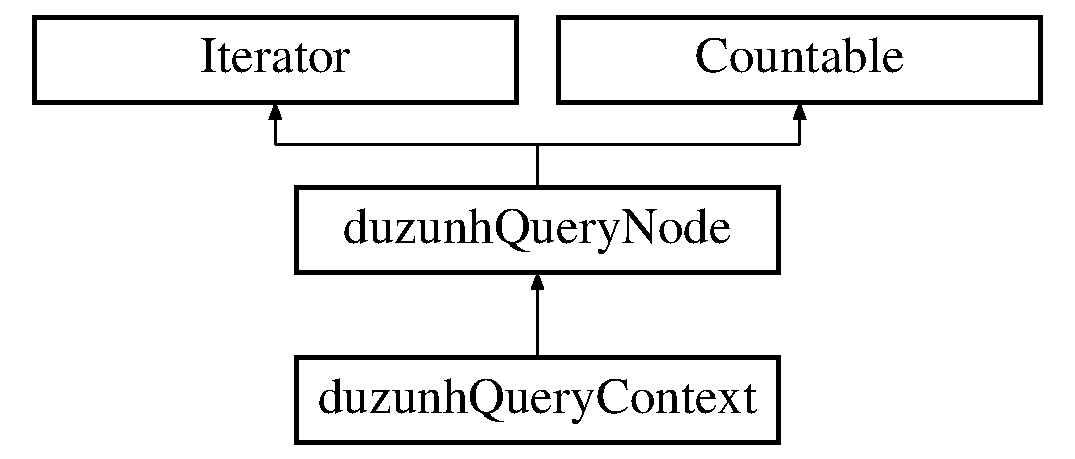
\includegraphics[height=3.000000cm]{classduzun_1_1hQuery_1_1Context}
\end{center}
\end{figure}
\subsection*{Public Member Functions}
\begin{DoxyCompactItemize}
\item 
\mbox{\Hypertarget{classduzun_1_1hQuery_1_1Context_a41294b6ffc5058da32d895bfcf4714b1}\label{classduzun_1_1hQuery_1_1Context_a41294b6ffc5058da32d895bfcf4714b1}} 
{\bfseries \+\_\+\+\_\+construct} (\$\mbox{\hyperlink{classduzun_1_1hQuery_1_1Node_abd060c044c66e49189d8e4fb491f3b3d}{doc}}=N\+U\+LL, \$el\+\_\+arr=N\+U\+LL)
\item 
\mbox{\hyperlink{classduzun_1_1hQuery_1_1Context_a8a3539a583a8e00f3bbd39b114b73542}{intersect}} (\$el, \$eq=true)
\end{DoxyCompactItemize}
\subsection*{Additional Inherited Members}


\subsection{Detailed Description}
A context is a list of node addresses with reference to their document.

A\+PI Documentation at \href{https://duzun.github.io/hQuery.php}{\tt https\+://duzun.\+github.\+io/h\+Query.\+php}

M\+IT 

Definition at line 16 of file Context.\+php.



\subsection{Member Function Documentation}
\mbox{\Hypertarget{classduzun_1_1hQuery_1_1Context_a8a3539a583a8e00f3bbd39b114b73542}\label{classduzun_1_1hQuery_1_1Context_a8a3539a583a8e00f3bbd39b114b73542}} 
\index{duzun\+::h\+Query\+::\+Context@{duzun\+::h\+Query\+::\+Context}!intersect@{intersect}}
\index{intersect@{intersect}!duzun\+::h\+Query\+::\+Context@{duzun\+::h\+Query\+::\+Context}}
\subsubsection{\texorpdfstring{intersect()}{intersect()}}
{\footnotesize\ttfamily duzun\textbackslash{}h\+Query\textbackslash{}\+Context\+::intersect (\begin{DoxyParamCaption}\item[{}]{\$el,  }\item[{}]{\$eq = {\ttfamily true} }\end{DoxyParamCaption})}

ctx(\$el) $\ast$ \$this

\begin{DoxyReturn}{Returns}
h\+Query\+\_\+\+Context ctx 
\end{DoxyReturn}


Definition at line 34 of file Context.\+php.



References duzun\textbackslash{}h\+Query\textbackslash{}\+Node\textbackslash{}\+\_\+ctx\+\_\+ids(), duzun\textbackslash{}h\+Query\textbackslash{}\+Node\textbackslash{}\+\_\+doc\+\_\+ids(), and duzun\textbackslash{}h\+Query\textbackslash{}\+Node\textbackslash{}\+\_\+has().



The documentation for this class was generated from the following file\+:\begin{DoxyCompactItemize}
\item 
src/h\+Query/Context.\+php\end{DoxyCompactItemize}

\hypertarget{classduzun_1_1hQuery_1_1Element}{}\section{duzun\textbackslash{}h\+Query\textbackslash{}Element Class Reference}
\label{classduzun_1_1hQuery_1_1Element}\index{duzun\textbackslash{}h\+Query\textbackslash{}\+Element@{duzun\textbackslash{}h\+Query\textbackslash{}\+Element}}
Inheritance diagram for duzun\textbackslash{}h\+Query\textbackslash{}Element\+:\begin{figure}[H]
\begin{center}
\leavevmode
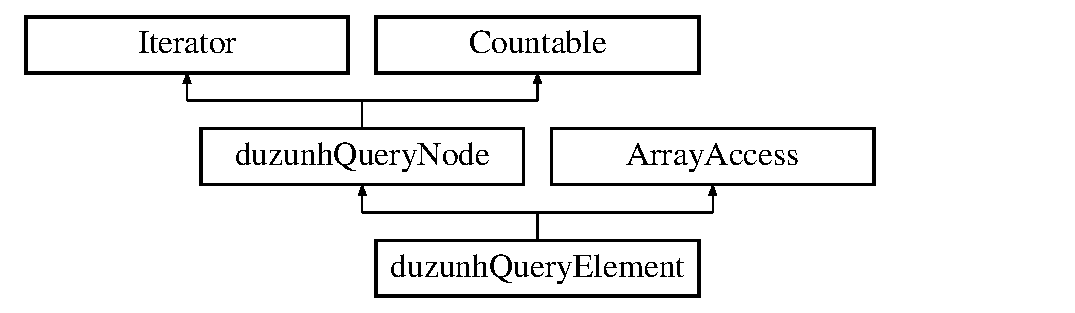
\includegraphics[height=3.000000cm]{classduzun_1_1hQuery_1_1Element}
\end{center}
\end{figure}
\subsection*{Public Member Functions}
\begin{DoxyCompactItemize}
\item 
\mbox{\Hypertarget{classduzun_1_1hQuery_1_1Element_a70cdd6880a13b65547ae89fedabc3686}\label{classduzun_1_1hQuery_1_1Element_a70cdd6880a13b65547ae89fedabc3686}} 
{\bfseries to\+Array} (\$cch=true)
\item 
\mbox{\Hypertarget{classduzun_1_1hQuery_1_1Element_a8480ff8371f157ce25a059b3c5ce5141}\label{classduzun_1_1hQuery_1_1Element_a8480ff8371f157ce25a059b3c5ce5141}} 
{\bfseries \+\_\+\+\_\+get} (\$name)
\item 
\mbox{\Hypertarget{classduzun_1_1hQuery_1_1Element_a9ad3dff6d3a73beb78cd718c7cfc302c}\label{classduzun_1_1hQuery_1_1Element_a9ad3dff6d3a73beb78cd718c7cfc302c}} 
{\bfseries offset\+Set} (\$offset, \$value)
\item 
\mbox{\Hypertarget{classduzun_1_1hQuery_1_1Element_aa4b03dbfae9b31f2c236c3ed958c9f7e}\label{classduzun_1_1hQuery_1_1Element_aa4b03dbfae9b31f2c236c3ed958c9f7e}} 
{\bfseries offset\+Get} (\$offset)
\item 
\mbox{\Hypertarget{classduzun_1_1hQuery_1_1Element_af681724466bfb37db382872d88f970d4}\label{classduzun_1_1hQuery_1_1Element_af681724466bfb37db382872d88f970d4}} 
{\bfseries offset\+Exists} (\$offset)
\item 
\mbox{\Hypertarget{classduzun_1_1hQuery_1_1Element_a201fa1e4b296059b4597bc0673ba2e50}\label{classduzun_1_1hQuery_1_1Element_a201fa1e4b296059b4597bc0673ba2e50}} 
{\bfseries offset\+Unset} (\$offset)
\item 
\mbox{\hyperlink{classduzun_1_1hQuery_1_1Element_abef85d8c18394f2c2c1fc25a4f439b55}{current}} ()
\item 
\mbox{\hyperlink{classduzun_1_1hQuery_1_1Element_a0ec6920ccb04c246df8490afeb89baf4}{val}} ()
\item 
\mbox{\hyperlink{classduzun_1_1hQuery_1_1Element_a0791de5ec50b8d91dacca06ee2074364}{has\+Class}} (\$class\+Name)
\item 
\mbox{\hyperlink{classduzun_1_1hQuery_1_1Element_aa629dd31a0d9ced799f65e4bd7c0b0f3}{get}} (\$idx)
\item 
\mbox{\hyperlink{classduzun_1_1hQuery_1_1Element_a2d857e83bcbd0d8de4c263b0afc64f43}{eq}} (\$idx)
\item 
\mbox{\hyperlink{classduzun_1_1hQuery_1_1Element_a172b277ee653f07905288411d20f42e5}{slice}} (\$idx, \$len=N\+U\+LL)
\item 
\mbox{\hyperlink{classduzun_1_1hQuery_1_1Element_a7a475b43ddf3e33b0d4fbc419d70369a}{parent}} ()
\item 
\mbox{\hyperlink{classduzun_1_1hQuery_1_1Element_ab19b0b422c54a00c0165543b5020253c}{children}} ()
\item 
\mbox{\hyperlink{classduzun_1_1hQuery_1_1Element_a189315f6240a6a76be142604c8258b27}{previous\+Element\+Sibling}} ()
\item 
\mbox{\hyperlink{classduzun_1_1hQuery_1_1Element_aae1431b6dd85e2289ce1b86ba9c9b4c5}{next\+Element\+Sibling}} ()
\end{DoxyCompactItemize}
\subsection*{Protected Attributes}
\begin{DoxyCompactItemize}
\item 
\mbox{\Hypertarget{classduzun_1_1hQuery_1_1Element_a8c6a560fddaeff4edca11742d328b20b}\label{classduzun_1_1hQuery_1_1Element_a8c6a560fddaeff4edca11742d328b20b}} 
{\bfseries \$\+\_\+ich} = N\+U\+LL
\end{DoxyCompactItemize}
\subsection*{Additional Inherited Members}


\subsection{Detailed Description}
Represents an H\+T\+ML \mbox{\hyperlink{classduzun_1_1hQuery_1_1Element}{Element}} ( eg div, input etc ) or a collection of elements ( eq j\+Query(\mbox{[}div, span, ...\mbox{]}) ) 

Definition at line 12 of file Element.\+php.



\subsection{Member Function Documentation}
\mbox{\Hypertarget{classduzun_1_1hQuery_1_1Element_ab19b0b422c54a00c0165543b5020253c}\label{classduzun_1_1hQuery_1_1Element_ab19b0b422c54a00c0165543b5020253c}} 
\index{duzun\+::h\+Query\+::\+Element@{duzun\+::h\+Query\+::\+Element}!children@{children}}
\index{children@{children}!duzun\+::h\+Query\+::\+Element@{duzun\+::h\+Query\+::\+Element}}
\subsubsection{\texorpdfstring{children()}{children()}}
{\footnotesize\ttfamily duzun\textbackslash{}h\+Query\textbackslash{}\+Element\+::children (\begin{DoxyParamCaption}{ }\end{DoxyParamCaption})}

Get child nodes for this collection of nodes.

\begin{DoxyReturn}{Returns}
h\+Query\+\_\+\+Element children 
\end{DoxyReturn}


Definition at line 254 of file Element.\+php.

\mbox{\Hypertarget{classduzun_1_1hQuery_1_1Element_abef85d8c18394f2c2c1fc25a4f439b55}\label{classduzun_1_1hQuery_1_1Element_abef85d8c18394f2c2c1fc25a4f439b55}} 
\index{duzun\+::h\+Query\+::\+Element@{duzun\+::h\+Query\+::\+Element}!current@{current}}
\index{current@{current}!duzun\+::h\+Query\+::\+Element@{duzun\+::h\+Query\+::\+Element}}
\subsubsection{\texorpdfstring{current()}{current()}}
{\footnotesize\ttfamily duzun\textbackslash{}h\+Query\textbackslash{}\+Element\+::current (\begin{DoxyParamCaption}{ }\end{DoxyParamCaption})}

Override \mbox{\hyperlink{classduzun_1_1hQuery_1_1Element_abef85d8c18394f2c2c1fc25a4f439b55}{current()}} for iterations.

\begin{DoxyReturn}{Returns}
h\+Query\+\_\+\+Element 
\end{DoxyReturn}


Definition at line 124 of file Element.\+php.

\mbox{\Hypertarget{classduzun_1_1hQuery_1_1Element_a2d857e83bcbd0d8de4c263b0afc64f43}\label{classduzun_1_1hQuery_1_1Element_a2d857e83bcbd0d8de4c263b0afc64f43}} 
\index{duzun\+::h\+Query\+::\+Element@{duzun\+::h\+Query\+::\+Element}!eq@{eq}}
\index{eq@{eq}!duzun\+::h\+Query\+::\+Element@{duzun\+::h\+Query\+::\+Element}}
\subsubsection{\texorpdfstring{eq()}{eq()}}
{\footnotesize\ttfamily duzun\textbackslash{}h\+Query\textbackslash{}\+Element\+::eq (\begin{DoxyParamCaption}\item[{}]{\$idx }\end{DoxyParamCaption})}

Get the node at \$idx position in the set, no cache, each call creates new instance.


\begin{DoxyParams}[1]{Parameters}
int & {\em \$idx} & -\/ index of an element, starts with 0.\\
\hline
\end{DoxyParams}
\begin{DoxyReturn}{Returns}
h\+Query\+\_\+\+Element 
\end{DoxyReturn}


Definition at line 200 of file Element.\+php.

\mbox{\Hypertarget{classduzun_1_1hQuery_1_1Element_aa629dd31a0d9ced799f65e4bd7c0b0f3}\label{classduzun_1_1hQuery_1_1Element_aa629dd31a0d9ced799f65e4bd7c0b0f3}} 
\index{duzun\+::h\+Query\+::\+Element@{duzun\+::h\+Query\+::\+Element}!get@{get}}
\index{get@{get}!duzun\+::h\+Query\+::\+Element@{duzun\+::h\+Query\+::\+Element}}
\subsubsection{\texorpdfstring{get()}{get()}}
{\footnotesize\ttfamily duzun\textbackslash{}h\+Query\textbackslash{}\+Element\+::get (\begin{DoxyParamCaption}\item[{}]{\$idx }\end{DoxyParamCaption})}

Get the node at \$idx position in the set, using cache


\begin{DoxyParams}[1]{Parameters}
int & {\em \$idx} & -\/ index of an element, starts with 0.\\
\hline
\end{DoxyParams}
\begin{DoxyReturn}{Returns}
h\+Query\+\_\+\+Element 
\end{DoxyReturn}


Definition at line 176 of file Element.\+php.

\mbox{\Hypertarget{classduzun_1_1hQuery_1_1Element_a0791de5ec50b8d91dacca06ee2074364}\label{classduzun_1_1hQuery_1_1Element_a0791de5ec50b8d91dacca06ee2074364}} 
\index{duzun\+::h\+Query\+::\+Element@{duzun\+::h\+Query\+::\+Element}!has\+Class@{has\+Class}}
\index{has\+Class@{has\+Class}!duzun\+::h\+Query\+::\+Element@{duzun\+::h\+Query\+::\+Element}}
\subsubsection{\texorpdfstring{has\+Class()}{hasClass()}}
{\footnotesize\ttfamily duzun\textbackslash{}h\+Query\textbackslash{}\+Element\+::has\+Class (\begin{DoxyParamCaption}\item[{}]{\$class\+Name }\end{DoxyParamCaption})}

Checks whether \$this element/collection has a(ll) class(es).


\begin{DoxyParams}[1]{Parameters}
string | array & {\em \$cl} & -\/ class(es) to check \\
\hline
\end{DoxyParams}
\begin{DoxyReturn}{Returns}
true -\/ has class, false -\/ no class, 0 -\/ doesn\textquotesingle{}t have any class, 
\end{DoxyReturn}


Definition at line 161 of file Element.\+php.



References duzun\textbackslash{}h\+Query\textbackslash{}\+Node\textbackslash{}doc().

\mbox{\Hypertarget{classduzun_1_1hQuery_1_1Element_aae1431b6dd85e2289ce1b86ba9c9b4c5}\label{classduzun_1_1hQuery_1_1Element_aae1431b6dd85e2289ce1b86ba9c9b4c5}} 
\index{duzun\+::h\+Query\+::\+Element@{duzun\+::h\+Query\+::\+Element}!next\+Element\+Sibling@{next\+Element\+Sibling}}
\index{next\+Element\+Sibling@{next\+Element\+Sibling}!duzun\+::h\+Query\+::\+Element@{duzun\+::h\+Query\+::\+Element}}
\subsubsection{\texorpdfstring{next\+Element\+Sibling()}{nextElementSibling()}}
{\footnotesize\ttfamily duzun\textbackslash{}h\+Query\textbackslash{}\+Element\+::next\+Element\+Sibling (\begin{DoxyParamCaption}{ }\end{DoxyParamCaption})}

Get next element siblings for each of the elements of this collection

\begin{DoxyReturn}{Returns}
h\+Query\+\_\+\+Element next\+Element\+Sibling 
\end{DoxyReturn}


Definition at line 274 of file Element.\+php.

\mbox{\Hypertarget{classduzun_1_1hQuery_1_1Element_a7a475b43ddf3e33b0d4fbc419d70369a}\label{classduzun_1_1hQuery_1_1Element_a7a475b43ddf3e33b0d4fbc419d70369a}} 
\index{duzun\+::h\+Query\+::\+Element@{duzun\+::h\+Query\+::\+Element}!parent@{parent}}
\index{parent@{parent}!duzun\+::h\+Query\+::\+Element@{duzun\+::h\+Query\+::\+Element}}
\subsubsection{\texorpdfstring{parent()}{parent()}}
{\footnotesize\ttfamily duzun\textbackslash{}h\+Query\textbackslash{}\+Element\+::parent (\begin{DoxyParamCaption}{ }\end{DoxyParamCaption})}

Get parent nodes for this collection of nodes.

\begin{DoxyReturn}{Returns}
h\+Query\+\_\+\+Element parent 
\end{DoxyReturn}


Definition at line 244 of file Element.\+php.

\mbox{\Hypertarget{classduzun_1_1hQuery_1_1Element_a189315f6240a6a76be142604c8258b27}\label{classduzun_1_1hQuery_1_1Element_a189315f6240a6a76be142604c8258b27}} 
\index{duzun\+::h\+Query\+::\+Element@{duzun\+::h\+Query\+::\+Element}!previous\+Element\+Sibling@{previous\+Element\+Sibling}}
\index{previous\+Element\+Sibling@{previous\+Element\+Sibling}!duzun\+::h\+Query\+::\+Element@{duzun\+::h\+Query\+::\+Element}}
\subsubsection{\texorpdfstring{previous\+Element\+Sibling()}{previousElementSibling()}}
{\footnotesize\ttfamily duzun\textbackslash{}h\+Query\textbackslash{}\+Element\+::previous\+Element\+Sibling (\begin{DoxyParamCaption}{ }\end{DoxyParamCaption})}

Get previous element siblings for each of the elements of this collection

\begin{DoxyReturn}{Returns}
h\+Query\+\_\+\+Element previous\+Element\+Sibling 
\end{DoxyReturn}


Definition at line 264 of file Element.\+php.

\mbox{\Hypertarget{classduzun_1_1hQuery_1_1Element_a172b277ee653f07905288411d20f42e5}\label{classduzun_1_1hQuery_1_1Element_a172b277ee653f07905288411d20f42e5}} 
\index{duzun\+::h\+Query\+::\+Element@{duzun\+::h\+Query\+::\+Element}!slice@{slice}}
\index{slice@{slice}!duzun\+::h\+Query\+::\+Element@{duzun\+::h\+Query\+::\+Element}}
\subsubsection{\texorpdfstring{slice()}{slice()}}
{\footnotesize\ttfamily duzun\textbackslash{}h\+Query\textbackslash{}\+Element\+::slice (\begin{DoxyParamCaption}\item[{}]{\$idx,  }\item[{}]{\$len = {\ttfamily NULL} }\end{DoxyParamCaption})}

Get a slice of current node collection.


\begin{DoxyParams}[1]{Parameters}
int & {\em \$idx} & -\/ start index of an element, starts with 0. \\
\hline
int & {\em \$len} & -\/ O\+P\+T\+I\+O\+N\+AL number of element to slice. Defaults to all starting at \$idx\\
\hline
\end{DoxyParams}
\begin{DoxyReturn}{Returns}
h\+Query\+\_\+\+Element 
\end{DoxyReturn}


Definition at line 216 of file Element.\+php.

\mbox{\Hypertarget{classduzun_1_1hQuery_1_1Element_a0ec6920ccb04c246df8490afeb89baf4}\label{classduzun_1_1hQuery_1_1Element_a0ec6920ccb04c246df8490afeb89baf4}} 
\index{duzun\+::h\+Query\+::\+Element@{duzun\+::h\+Query\+::\+Element}!val@{val}}
\index{val@{val}!duzun\+::h\+Query\+::\+Element@{duzun\+::h\+Query\+::\+Element}}
\subsubsection{\texorpdfstring{val()}{val()}}
{\footnotesize\ttfamily duzun\textbackslash{}h\+Query\textbackslash{}\+Element\+::val (\begin{DoxyParamCaption}{ }\end{DoxyParamCaption})}

Get value of an \+:input element.

\begin{DoxyReturn}{Returns}
mixed value of the first element in the collection. 
\end{DoxyReturn}


Definition at line 138 of file Element.\+php.



The documentation for this class was generated from the following file\+:\begin{DoxyCompactItemize}
\item 
src/h\+Query/Element.\+php\end{DoxyCompactItemize}

\hypertarget{classduzun_1_1hQuery}{}\section{duzun\textbackslash{}h\+Query Class Reference}
\label{classduzun_1_1hQuery}\index{duzun\textbackslash{}h\+Query@{duzun\textbackslash{}h\+Query}}
Inheritance diagram for duzun\textbackslash{}h\+Query\+:\begin{figure}[H]
\begin{center}
\leavevmode
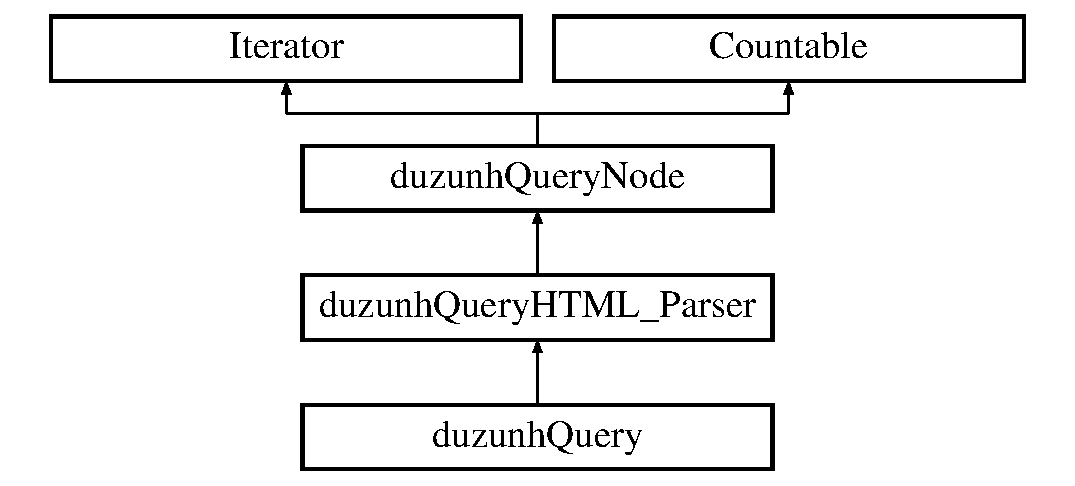
\includegraphics[height=4.000000cm]{classduzun_1_1hQuery}
\end{center}
\end{figure}
\subsection*{Public Member Functions}
\begin{DoxyCompactItemize}
\item 
\mbox{\hyperlink{classduzun_1_1hQuery_a3565bdeabc08bd32d10d365759e9dc82}{find}} (\$sel, \$\+\_\+attr=N\+U\+LL, \$ctx=N\+U\+LL)
\item 
\mbox{\hyperlink{classduzun_1_1hQuery_ac8332727e97405b17ecb4dd47c5a0fc9}{find\+\_\+html}} (\$sel, \$\mbox{\hyperlink{classduzun_1_1hQuery_1_1Node_a530ab9e8edeb1e876b369dcb321208c0}{attr}}=N\+U\+LL, \$ctx=N\+U\+LL)
\item 
\mbox{\hyperlink{classduzun_1_1hQuery_a3d00fababd6c54d00ee89a562233730d}{find\+\_\+text}} (\$sel, \$\mbox{\hyperlink{classduzun_1_1hQuery_1_1Node_a530ab9e8edeb1e876b369dcb321208c0}{attr}}=N\+U\+LL, \$ctx=N\+U\+LL)
\item 
\mbox{\hyperlink{classduzun_1_1hQuery_adf6b1bc1eb43a8e88effc0662e2edc49}{index}} ()
\end{DoxyCompactItemize}
\subsection*{Static Public Member Functions}
\begin{DoxyCompactItemize}
\item 
static \mbox{\hyperlink{classduzun_1_1hQuery_a00c55ba68b55dc033bea74623927ca0f}{from\+H\+T\+ML}} (\$\mbox{\hyperlink{classduzun_1_1hQuery_1_1Node_a6a251f5f93690fabb794c673388dd49b}{html}}, \$url=N\+U\+LL)
\item 
static \mbox{\hyperlink{classduzun_1_1hQuery_a68c406e030e2ccd85707c20c2eedf720}{from\+File}} (\$filename, \$use\+\_\+include\+\_\+path=false, \$context=N\+U\+LL)
\item 
static \mbox{\hyperlink{classduzun_1_1hQuery_a2e7353a5236495ec6c29e68037a86438}{from\+U\+RL}} (\$url, \$headers=N\+U\+LL, \$body=N\+U\+LL, \$options=N\+U\+LL)
\item 
static \mbox{\hyperlink{classduzun_1_1hQuery_a6af08d4cefbb0d2184ff90377f6f757f}{jsonize}} (\$data, \&\$type=N\+U\+LL, \$ops=0)
\item 
static \mbox{\hyperlink{classduzun_1_1hQuery_af5457644a63722ff789fababb88e99c5}{unjsonize}} (\$str, \&\$type=N\+U\+LL)
\item 
static \mbox{\hyperlink{classduzun_1_1hQuery_ad991b9626160044464a687ee32bd61c5}{gz\+\_\+supported}} ()
\item 
static \mbox{\hyperlink{classduzun_1_1hQuery_a84f0b53d5a2ae0e695a49f5b0f85c857}{gzdecode}} (\$str)
\item 
static \mbox{\hyperlink{classduzun_1_1hQuery_a5326810be6da35a2567137787be41ada}{do\+\_\+flock}} (\$fp, \$lock, \$timeout\+\_\+ms=384)
\item 
\mbox{\Hypertarget{classduzun_1_1hQuery_a8ef4d640cfeb8c0e88b34a056195b53e}\label{classduzun_1_1hQuery_a8ef4d640cfeb8c0e88b34a056195b53e}} 
static {\bfseries flock\+\_\+put\+\_\+contents} (\$fn, \$cnt, \$block=false)
\item 
\mbox{\Hypertarget{classduzun_1_1hQuery_a1d63a8628bdf1a94d0600dff9514eca9}\label{classduzun_1_1hQuery_a1d63a8628bdf1a94d0600dff9514eca9}} 
static {\bfseries flock\+\_\+get\+\_\+contents} (\$fn, \$block=false)
\item 
\mbox{\Hypertarget{classduzun_1_1hQuery_a2dc9003ba3cef6852dc4321c63c4ffce}\label{classduzun_1_1hQuery_a2dc9003ba3cef6852dc4321c63c4ffce}} 
static {\bfseries parse\+\_\+cookie} (\$str)
\item 
static \mbox{\hyperlink{classduzun_1_1hQuery_af3a116011d32dbaa4efe6ff10c0f608f}{http\+\_\+wr}} (\$host, \$head=N\+U\+LL, \$body=N\+U\+LL, \$options=N\+U\+LL)
\end{DoxyCompactItemize}
\subsection*{Public Attributes}
\begin{DoxyCompactItemize}
\item 
\mbox{\Hypertarget{classduzun_1_1hQuery_a83d15ffbefcbf2459bf50bb10ed79514}\label{classduzun_1_1hQuery_a83d15ffbefcbf2459bf50bb10ed79514}} 
{\bfseries \$headers}
\end{DoxyCompactItemize}
\subsection*{Static Public Attributes}
\begin{DoxyCompactItemize}
\item 
\mbox{\Hypertarget{classduzun_1_1hQuery_a2a97f056a6ce83b7c6016e25cf2538e4}\label{classduzun_1_1hQuery_a2a97f056a6ce83b7c6016e25cf2538e4}} 
static {\bfseries \$cache\+\_\+path}
\item 
\mbox{\Hypertarget{classduzun_1_1hQuery_a34e4d9410985fd7cde08ba84892084e3}\label{classduzun_1_1hQuery_a34e4d9410985fd7cde08ba84892084e3}} 
static {\bfseries \$cache\+\_\+expires} = 3600
\item 
\mbox{\Hypertarget{classduzun_1_1hQuery_af47ffc7fdf974e3e0d109f426be39a74}\label{classduzun_1_1hQuery_af47ffc7fdf974e3e0d109f426be39a74}} 
static {\bfseries \$\+\_\+mockup\+\_\+class}
\end{DoxyCompactItemize}
\subsection*{Static Protected Member Functions}
\begin{DoxyCompactItemize}
\item 
static \mbox{\hyperlink{classduzun_1_1hQuery_ac01b0ddd586fe833f61c733147231a47}{serjstype}} (\$str)
\item 
static \mbox{\hyperlink{classduzun_1_1hQuery_a91deb0634713a3471cd5101b8b66b579}{\+\_\+gzdecode}} (\$gzdata, \$maxlen=N\+U\+LL)
\item 
static \mbox{\hyperlink{classduzun_1_1hQuery_a3b0cda49e9c7695c2fc88f3ad1657c61}{get\+\_\+cache}} (\$fn, \$expire=false, \$meta\+\_\+only=false)
\item 
static \mbox{\hyperlink{classduzun_1_1hQuery_a9e61ec098daddf504ffc239ff7d7910f}{set\+\_\+cache}} (\$fn, \$cnt, \$meta=N\+U\+LL, \$gzip=true)
\end{DoxyCompactItemize}
\subsection*{Additional Inherited Members}


\subsection{Detailed Description}
Main Class, represents an H\+T\+ML document.

An extremely fast web scraper that parses megabytes of H\+T\+ML in a blink of an eye. P\+H\+P5+, no dependencies.

A\+PI Documentation at \href{https://duzun.github.io/hQuery.php}{\tt https\+://duzun.\+github.\+io/h\+Query.\+php}

Copyright (C) 2014-\/2018 Dumitru Uzun

\begin{DoxyAuthor}{Author}
Dumitru Uzun (D\+Uzun.\+ME)  M\+IT 
\end{DoxyAuthor}
\begin{DoxyVersion}{Version}
2.\+0.\+2 
\end{DoxyVersion}


Definition at line 21 of file h\+Query.\+php.



\subsection{Member Function Documentation}
\mbox{\Hypertarget{classduzun_1_1hQuery_a91deb0634713a3471cd5101b8b66b579}\label{classduzun_1_1hQuery_a91deb0634713a3471cd5101b8b66b579}} 
\index{duzun\+::h\+Query@{duzun\+::h\+Query}!\+\_\+gzdecode@{\+\_\+gzdecode}}
\index{\+\_\+gzdecode@{\+\_\+gzdecode}!duzun\+::h\+Query@{duzun\+::h\+Query}}
\subsubsection{\texorpdfstring{\+\_\+gzdecode()}{\_gzdecode()}}
{\footnotesize\ttfamily static duzun\textbackslash{}h\+Query\+::\+\_\+gzdecode (\begin{DoxyParamCaption}\item[{}]{\$gzdata,  }\item[{}]{\$maxlen = {\ttfamily NULL} }\end{DoxyParamCaption})\hspace{0.3cm}{\ttfamily [static]}, {\ttfamily [protected]}}

Alternative \mbox{\hyperlink{classduzun_1_1hQuery_a84f0b53d5a2ae0e695a49f5b0f85c857}{gzdecode()}} (for P\+HP $<$ 5.\+4.\+0) source\+: \href{https://github.com/Polycademy/upgradephp/blob/master/upgrade.php}{\tt https\+://github.\+com/\+Polycademy/upgradephp/blob/master/upgrade.\+php} 

Definition at line 458 of file h\+Query.\+php.

\mbox{\Hypertarget{classduzun_1_1hQuery_a5326810be6da35a2567137787be41ada}\label{classduzun_1_1hQuery_a5326810be6da35a2567137787be41ada}} 
\index{duzun\+::h\+Query@{duzun\+::h\+Query}!do\+\_\+flock@{do\+\_\+flock}}
\index{do\+\_\+flock@{do\+\_\+flock}!duzun\+::h\+Query@{duzun\+::h\+Query}}
\subsubsection{\texorpdfstring{do\+\_\+flock()}{do\_flock()}}
{\footnotesize\ttfamily static duzun\textbackslash{}h\+Query\+::do\+\_\+flock (\begin{DoxyParamCaption}\item[{}]{\$fp,  }\item[{}]{\$lock,  }\item[{}]{\$timeout\+\_\+ms = {\ttfamily 384} }\end{DoxyParamCaption})\hspace{0.3cm}{\ttfamily [static]}}

Lock with retries


\begin{DoxyParams}[1]{Parameters}
resource & {\em \$fp} & -\/ Open file pointer \\
\hline
int & {\em \$lock} & -\/ Lock type \\
\hline
int & {\em \$timeout\+\_\+ms} & -\/ O\+P\+T\+I\+O\+N\+AL Timeout to wait for unlock in miliseconds\\
\hline
\end{DoxyParams}
\begin{DoxyReturn}{Returns}
true on success, false on fail
\end{DoxyReturn}
\begin{DoxyAuthor}{Author}
Dumitru Uzun 
\end{DoxyAuthor}


Definition at line 611 of file h\+Query.\+php.

\mbox{\Hypertarget{classduzun_1_1hQuery_a3565bdeabc08bd32d10d365759e9dc82}\label{classduzun_1_1hQuery_a3565bdeabc08bd32d10d365759e9dc82}} 
\index{duzun\+::h\+Query@{duzun\+::h\+Query}!find@{find}}
\index{find@{find}!duzun\+::h\+Query@{duzun\+::h\+Query}}
\subsubsection{\texorpdfstring{find()}{find()}}
{\footnotesize\ttfamily duzun\textbackslash{}h\+Query\+::find (\begin{DoxyParamCaption}\item[{}]{\$sel,  }\item[{}]{\$\+\_\+attr = {\ttfamily NULL},  }\item[{}]{\$ctx = {\ttfamily NULL} }\end{DoxyParamCaption})}

Finds a collection of nodes inside current document/context (similar to j\+Query.\+fn.\+find()).


\begin{DoxyParams}[1]{Parameters}
string & {\em \$sel} & -\/ A valid C\+SS selector (some pseudo-\/selectors supported). \\
\hline
array | string & {\em \$attr} & -\/ O\+P\+T\+I\+O\+N\+AL attributes as string or key-\/value pairs. \\
\hline
h\+Query\textbackslash{}\+Node & {\em \$ctx} & -\/ O\+P\+T\+I\+O\+N\+AL the context where to search. If omitted, \$this is used.\\
\hline
\end{DoxyParams}
\begin{DoxyReturn}{Returns}
\mbox{\hyperlink{classduzun_1_1hQuery}{h\+Query}} collection of matched elements or N\+U\+LL 
\end{DoxyReturn}


Definition at line 182 of file h\+Query.\+php.



Referenced by duzun\textbackslash{}h\+Query\textbackslash{}\+H\+T\+M\+L\+\_\+\+Parser\textbackslash{}has\+Class().

\mbox{\Hypertarget{classduzun_1_1hQuery_ac8332727e97405b17ecb4dd47c5a0fc9}\label{classduzun_1_1hQuery_ac8332727e97405b17ecb4dd47c5a0fc9}} 
\index{duzun\+::h\+Query@{duzun\+::h\+Query}!find\+\_\+html@{find\+\_\+html}}
\index{find\+\_\+html@{find\+\_\+html}!duzun\+::h\+Query@{duzun\+::h\+Query}}
\subsubsection{\texorpdfstring{find\+\_\+html()}{find\_html()}}
{\footnotesize\ttfamily duzun\textbackslash{}h\+Query\+::find\+\_\+html (\begin{DoxyParamCaption}\item[{}]{\$sel,  }\item[{}]{\$attr = {\ttfamily NULL},  }\item[{}]{\$ctx = {\ttfamily NULL} }\end{DoxyParamCaption})}

Combination of -\/$>$\mbox{\hyperlink{classduzun_1_1hQuery_a3565bdeabc08bd32d10d365759e9dc82}{find()}} + -\/$>$\mbox{\hyperlink{classduzun_1_1hQuery_1_1Node_a6a251f5f93690fabb794c673388dd49b}{html()}}


\begin{DoxyParams}[1]{Parameters}
string & {\em \$sel} & -\/ A valid C\+SS selector. \\
\hline
array | string & {\em \$attr} & -\/ O\+P\+T\+I\+O\+N\+AL attributes as string or key-\/value pairs. \\
\hline
h\+Query\textbackslash{}\+Node & {\em \$ctx} & -\/ O\+P\+T\+I\+O\+N\+AL the context where to search. If omitted, \$this is used.\\
\hline
\end{DoxyParams}
\begin{DoxyReturn}{Returns}
array list of H\+T\+ML contents of all matched elements 
\end{DoxyReturn}


Definition at line 269 of file h\+Query.\+php.

\mbox{\Hypertarget{classduzun_1_1hQuery_a3d00fababd6c54d00ee89a562233730d}\label{classduzun_1_1hQuery_a3d00fababd6c54d00ee89a562233730d}} 
\index{duzun\+::h\+Query@{duzun\+::h\+Query}!find\+\_\+text@{find\+\_\+text}}
\index{find\+\_\+text@{find\+\_\+text}!duzun\+::h\+Query@{duzun\+::h\+Query}}
\subsubsection{\texorpdfstring{find\+\_\+text()}{find\_text()}}
{\footnotesize\ttfamily duzun\textbackslash{}h\+Query\+::find\+\_\+text (\begin{DoxyParamCaption}\item[{}]{\$sel,  }\item[{}]{\$attr = {\ttfamily NULL},  }\item[{}]{\$ctx = {\ttfamily NULL} }\end{DoxyParamCaption})}

Combination of -\/$>$\mbox{\hyperlink{classduzun_1_1hQuery_a3565bdeabc08bd32d10d365759e9dc82}{find()}} + -\/$>$\mbox{\hyperlink{classduzun_1_1hQuery_1_1Node_ad5395ffe77dd4f111fcc7f59d211fbfa}{text()}}


\begin{DoxyParams}[1]{Parameters}
string & {\em \$sel} & -\/ A valid C\+SS selector. \\
\hline
array | string & {\em \$attr} & -\/ O\+P\+T\+I\+O\+N\+AL attributes as string or key-\/value pairs. \\
\hline
h\+Query\textbackslash{}\+Node & {\em \$ctx} & -\/ O\+P\+T\+I\+O\+N\+AL the context where to search. If omitted, \$this is used.\\
\hline
\end{DoxyParams}
\begin{DoxyReturn}{Returns}
array list of Text contents of all matched elements 
\end{DoxyReturn}


Definition at line 285 of file h\+Query.\+php.

\mbox{\Hypertarget{classduzun_1_1hQuery_a68c406e030e2ccd85707c20c2eedf720}\label{classduzun_1_1hQuery_a68c406e030e2ccd85707c20c2eedf720}} 
\index{duzun\+::h\+Query@{duzun\+::h\+Query}!from\+File@{from\+File}}
\index{from\+File@{from\+File}!duzun\+::h\+Query@{duzun\+::h\+Query}}
\subsubsection{\texorpdfstring{from\+File()}{fromFile()}}
{\footnotesize\ttfamily static duzun\textbackslash{}h\+Query\+::from\+File (\begin{DoxyParamCaption}\item[{}]{\$filename,  }\item[{}]{\$use\+\_\+include\+\_\+path = {\ttfamily false},  }\item[{}]{\$context = {\ttfamily NULL} }\end{DoxyParamCaption})\hspace{0.3cm}{\ttfamily [static]}}

Read the H\+T\+ML document from a file.


\begin{DoxyParams}[1]{Parameters}
string & {\em \$filename} & -\/ a valid filename \\
\hline
bool & {\em \$use\+\_\+include\+\_\+path} & -\/ O\+P\+T\+I\+O\+N\+AL passed to file\+\_\+get\+\_\+contents() \\
\hline
resource & {\em \$context} & -\/ O\+P\+T\+I\+O\+N\+AL A valid context resource created with stream\+\_\+context\+\_\+create(). See file\+\_\+get\+\_\+contents()\\
\hline
\end{DoxyParams}
\begin{DoxyReturn}{Returns}
\mbox{\hyperlink{classduzun_1_1hQuery}{h\+Query}} \$doc 
\end{DoxyReturn}


Definition at line 67 of file h\+Query.\+php.

\mbox{\Hypertarget{classduzun_1_1hQuery_a00c55ba68b55dc033bea74623927ca0f}\label{classduzun_1_1hQuery_a00c55ba68b55dc033bea74623927ca0f}} 
\index{duzun\+::h\+Query@{duzun\+::h\+Query}!from\+H\+T\+ML@{from\+H\+T\+ML}}
\index{from\+H\+T\+ML@{from\+H\+T\+ML}!duzun\+::h\+Query@{duzun\+::h\+Query}}
\subsubsection{\texorpdfstring{from\+H\+T\+M\+L()}{fromHTML()}}
{\footnotesize\ttfamily static duzun\textbackslash{}h\+Query\+::from\+H\+T\+ML (\begin{DoxyParamCaption}\item[{}]{\$html,  }\item[{}]{\$url = {\ttfamily NULL} }\end{DoxyParamCaption})\hspace{0.3cm}{\ttfamily [static]}}

Parse and H\+T\+ML string.


\begin{DoxyParams}[1]{Parameters}
string & {\em \$html} & -\/ source of some H\+T\+ML document \\
\hline
string & {\em \$url} & -\/ O\+P\+T\+I\+O\+N\+AL location of the document. Used for relative U\+R\+Ls inside the document.\\
\hline
\end{DoxyParams}
\begin{DoxyReturn}{Returns}
\mbox{\hyperlink{classduzun_1_1hQuery}{h\+Query}} \$doc 
\end{DoxyReturn}


Definition at line 41 of file h\+Query.\+php.

\mbox{\Hypertarget{classduzun_1_1hQuery_a2e7353a5236495ec6c29e68037a86438}\label{classduzun_1_1hQuery_a2e7353a5236495ec6c29e68037a86438}} 
\index{duzun\+::h\+Query@{duzun\+::h\+Query}!from\+U\+RL@{from\+U\+RL}}
\index{from\+U\+RL@{from\+U\+RL}!duzun\+::h\+Query@{duzun\+::h\+Query}}
\subsubsection{\texorpdfstring{from\+U\+R\+L()}{fromURL()}}
{\footnotesize\ttfamily static duzun\textbackslash{}h\+Query\+::from\+U\+RL (\begin{DoxyParamCaption}\item[{}]{\$url,  }\item[{}]{\$headers = {\ttfamily NULL},  }\item[{}]{\$body = {\ttfamily NULL},  }\item[{}]{\$options = {\ttfamily NULL} }\end{DoxyParamCaption})\hspace{0.3cm}{\ttfamily [static]}}

Fetch the H\+T\+ML document from remote \$url.


\begin{DoxyParams}[1]{Parameters}
string & {\em \$url} & -\/ the U\+RL of the document \\
\hline
array & {\em \$headers} & -\/ O\+P\+T\+I\+O\+N\+AL request headers \\
\hline
array | string & {\em \$body} & -\/ O\+P\+T\+I\+O\+N\+AL body of the request (for P\+O\+ST or P\+UT) \\
\hline
array & {\em \$options} & -\/ O\+P\+T\+I\+O\+N\+AL request options (see self\+::http\+\_\+wr() for more details)\\
\hline
\end{DoxyParams}
\begin{DoxyReturn}{Returns}
\mbox{\hyperlink{classduzun_1_1hQuery}{h\+Query}} \$doc 
\end{DoxyReturn}


Definition at line 88 of file h\+Query.\+php.

\mbox{\Hypertarget{classduzun_1_1hQuery_a3b0cda49e9c7695c2fc88f3ad1657c61}\label{classduzun_1_1hQuery_a3b0cda49e9c7695c2fc88f3ad1657c61}} 
\index{duzun\+::h\+Query@{duzun\+::h\+Query}!get\+\_\+cache@{get\+\_\+cache}}
\index{get\+\_\+cache@{get\+\_\+cache}!duzun\+::h\+Query@{duzun\+::h\+Query}}
\subsubsection{\texorpdfstring{get\+\_\+cache()}{get\_cache()}}
{\footnotesize\ttfamily static duzun\textbackslash{}h\+Query\+::get\+\_\+cache (\begin{DoxyParamCaption}\item[{}]{\$fn,  }\item[{}]{\$expire = {\ttfamily false},  }\item[{}]{\$meta\+\_\+only = {\ttfamily false} }\end{DoxyParamCaption})\hspace{0.3cm}{\ttfamily [static]}, {\ttfamily [protected]}}

Read data from a cache file.


\begin{DoxyParams}[1]{Parameters}
string & {\em \$fn} & -\/ cache filename \\
\hline
int & {\em \$expire} & -\/ O\+P\+T\+I\+O\+N\+AL contents returned only if it is newer then \$expire seconds \\
\hline
bool & {\em \$meta\+\_\+only} & -\/ O\+P\+T\+I\+O\+N\+AL if T\+R\+UE, read only meta-\/info (faster)\\
\hline
\end{DoxyParams}
\begin{DoxyReturn}{Returns}
array \mbox{[}mixed $<$contents$>$, array $<$meta\+\_\+info$>$\mbox{]} 
\end{DoxyReturn}


Definition at line 532 of file h\+Query.\+php.

\mbox{\Hypertarget{classduzun_1_1hQuery_ad991b9626160044464a687ee32bd61c5}\label{classduzun_1_1hQuery_ad991b9626160044464a687ee32bd61c5}} 
\index{duzun\+::h\+Query@{duzun\+::h\+Query}!gz\+\_\+supported@{gz\+\_\+supported}}
\index{gz\+\_\+supported@{gz\+\_\+supported}!duzun\+::h\+Query@{duzun\+::h\+Query}}
\subsubsection{\texorpdfstring{gz\+\_\+supported()}{gz\_supported()}}
{\footnotesize\ttfamily static duzun\textbackslash{}h\+Query\+::gz\+\_\+supported (\begin{DoxyParamCaption}{ }\end{DoxyParamCaption})\hspace{0.3cm}{\ttfamily [static]}}

Find a function to decode gzip data. \begin{DoxyReturn}{Returns}
string A gzip decode function name, or false if not found 
\end{DoxyReturn}


Definition at line 435 of file h\+Query.\+php.

\mbox{\Hypertarget{classduzun_1_1hQuery_a84f0b53d5a2ae0e695a49f5b0f85c857}\label{classduzun_1_1hQuery_a84f0b53d5a2ae0e695a49f5b0f85c857}} 
\index{duzun\+::h\+Query@{duzun\+::h\+Query}!gzdecode@{gzdecode}}
\index{gzdecode@{gzdecode}!duzun\+::h\+Query@{duzun\+::h\+Query}}
\subsubsection{\texorpdfstring{gzdecode()}{gzdecode()}}
{\footnotesize\ttfamily static duzun\textbackslash{}h\+Query\+::gzdecode (\begin{DoxyParamCaption}\item[{}]{\$str }\end{DoxyParamCaption})\hspace{0.3cm}{\ttfamily [static]}}

\mbox{\hyperlink{classduzun_1_1hQuery_a84f0b53d5a2ae0e695a49f5b0f85c857}{gzdecode()}} (for P\+HP $<$ 5.\+4.\+0) 

Definition at line 445 of file h\+Query.\+php.

\mbox{\Hypertarget{classduzun_1_1hQuery_af3a116011d32dbaa4efe6ff10c0f608f}\label{classduzun_1_1hQuery_af3a116011d32dbaa4efe6ff10c0f608f}} 
\index{duzun\+::h\+Query@{duzun\+::h\+Query}!http\+\_\+wr@{http\+\_\+wr}}
\index{http\+\_\+wr@{http\+\_\+wr}!duzun\+::h\+Query@{duzun\+::h\+Query}}
\subsubsection{\texorpdfstring{http\+\_\+wr()}{http\_wr()}}
{\footnotesize\ttfamily static duzun\textbackslash{}h\+Query\+::http\+\_\+wr (\begin{DoxyParamCaption}\item[{}]{\$host,  }\item[{}]{\$head = {\ttfamily NULL},  }\item[{}]{\$body = {\ttfamily NULL},  }\item[{}]{\$options = {\ttfamily NULL} }\end{DoxyParamCaption})\hspace{0.3cm}{\ttfamily [static]}}

Executes a H\+T\+TP write-\/read session.


\begin{DoxyParams}[1]{Parameters}
string & {\em \$host} & -\/ I\+P/\+H\+O\+ST address or U\+RL \\
\hline
array & {\em \$head} & -\/ list off H\+T\+TP headers to be sent along with the request to \$host \\
\hline
mixed & {\em \$body} & -\/ data to be sent as the contents of the request. If is array or object, a http query is built. \\
\hline
array & {\em \$options} & -\/ list of option as key-\/value\+: timeout -\/ connection timeout in seconds host -\/ goes to headers, overrides \$host (ex. \$host == \textquotesingle{}127.\+0.\+0.\+1\textquotesingle{}, \$options\mbox{[}\textquotesingle{}host\textquotesingle{}\mbox{]} == \textquotesingle{}www.\+example.\+com\textquotesingle{}) port -\/ usefull when \$host is not a full U\+RL scheme -\/ http, ssl, tls, udp, ... close -\/ whether to close connection o not redirects -\/ number of allowed redirects redirect\+\_\+method -\/ if (string), this is the new method for redirect request, else if true, preserve method, else use \textquotesingle{}G\+ET\textquotesingle{} on redirect. by default preserve on 307 and 308, G\+ET on 301-\/303\\
\hline
\end{DoxyParams}
\begin{DoxyReturn}{Returns}
array \mbox{[}contents, headers, http-\/status-\/code, http-\/status-\/message\mbox{]}
\end{DoxyReturn}
\begin{DoxyAuthor}{Author}
Dumitru Uzun 
\end{DoxyAuthor}


Definition at line 720 of file h\+Query.\+php.

\mbox{\Hypertarget{classduzun_1_1hQuery_adf6b1bc1eb43a8e88effc0662e2edc49}\label{classduzun_1_1hQuery_adf6b1bc1eb43a8e88effc0662e2edc49}} 
\index{duzun\+::h\+Query@{duzun\+::h\+Query}!index@{index}}
\index{index@{index}!duzun\+::h\+Query@{duzun\+::h\+Query}}
\subsubsection{\texorpdfstring{index()}{index()}}
{\footnotesize\ttfamily duzun\textbackslash{}h\+Query\+::index (\begin{DoxyParamCaption}{ }\end{DoxyParamCaption})}

Index elements of the source H\+T\+ML. (Called automatically) 

Definition at line 295 of file h\+Query.\+php.

\mbox{\Hypertarget{classduzun_1_1hQuery_a6af08d4cefbb0d2184ff90377f6f757f}\label{classduzun_1_1hQuery_a6af08d4cefbb0d2184ff90377f6f757f}} 
\index{duzun\+::h\+Query@{duzun\+::h\+Query}!jsonize@{jsonize}}
\index{jsonize@{jsonize}!duzun\+::h\+Query@{duzun\+::h\+Query}}
\subsubsection{\texorpdfstring{jsonize()}{jsonize()}}
{\footnotesize\ttfamily static duzun\textbackslash{}h\+Query\+::jsonize (\begin{DoxyParamCaption}\item[{}]{\$data,  }\item[{\&}]{\$type = {\ttfamily NULL},  }\item[{}]{\$ops = {\ttfamily 0} }\end{DoxyParamCaption})\hspace{0.3cm}{\ttfamily [static]}}

Serialize \$data as J\+S\+ON, fallback to serialize.


\begin{DoxyParams}[1]{Parameters}
mixed & {\em \$data} & -\/ the data to be serialized \\
\hline
 & {\em \&string} & \$type -\/ returns the serialization method used (\textquotesingle{}json\textquotesingle{} $\vert$ \textquotesingle{}ser\textquotesingle{})\\
\hline
\end{DoxyParams}
\begin{DoxyReturn}{Returns}
string the serialized data 
\end{DoxyReturn}


Definition at line 308 of file h\+Query.\+php.

\mbox{\Hypertarget{classduzun_1_1hQuery_ac01b0ddd586fe833f61c733147231a47}\label{classduzun_1_1hQuery_ac01b0ddd586fe833f61c733147231a47}} 
\index{duzun\+::h\+Query@{duzun\+::h\+Query}!serjstype@{serjstype}}
\index{serjstype@{serjstype}!duzun\+::h\+Query@{duzun\+::h\+Query}}
\subsubsection{\texorpdfstring{serjstype()}{serjstype()}}
{\footnotesize\ttfamily static duzun\textbackslash{}h\+Query\+::serjstype (\begin{DoxyParamCaption}\item[{}]{\$str }\end{DoxyParamCaption})\hspace{0.3cm}{\ttfamily [static]}, {\ttfamily [protected]}}

Tries to detect format of \$str (json or ser).


\begin{DoxyParams}[1]{Parameters}
string & {\em \$str} & -\/ J\+S\+ON encoded or P\+HP serialized data.\\
\hline
\end{DoxyParams}
\begin{DoxyReturn}{Returns}
string \textquotesingle{}json\textquotesingle{} $\vert$ \textquotesingle{}ser\textquotesingle{}, or F\+A\+L\+SE on failure to detect format. 
\end{DoxyReturn}


Definition at line 414 of file h\+Query.\+php.

\mbox{\Hypertarget{classduzun_1_1hQuery_a9e61ec098daddf504ffc239ff7d7910f}\label{classduzun_1_1hQuery_a9e61ec098daddf504ffc239ff7d7910f}} 
\index{duzun\+::h\+Query@{duzun\+::h\+Query}!set\+\_\+cache@{set\+\_\+cache}}
\index{set\+\_\+cache@{set\+\_\+cache}!duzun\+::h\+Query@{duzun\+::h\+Query}}
\subsubsection{\texorpdfstring{set\+\_\+cache()}{set\_cache()}}
{\footnotesize\ttfamily static duzun\textbackslash{}h\+Query\+::set\+\_\+cache (\begin{DoxyParamCaption}\item[{}]{\$fn,  }\item[{}]{\$cnt,  }\item[{}]{\$meta = {\ttfamily NULL},  }\item[{}]{\$gzip = {\ttfamily true} }\end{DoxyParamCaption})\hspace{0.3cm}{\ttfamily [static]}, {\ttfamily [protected]}}

Save data to a cache file.


\begin{DoxyParams}[1]{Parameters}
string & {\em \$fn} & -\/ cache filename \\
\hline
mixed & {\em \$cnt} & -\/ contents to be cached \\
\hline
array & {\em \$meta} & -\/ O\+P\+T\+I\+O\+N\+AL meta information related to contents. \\
\hline
bool & {\em \$gzip} & -\/ O\+P\+T\+I\+O\+N\+AL if T\+R\+UE and gzip supported, store contents gzipped\\
\hline
\end{DoxyParams}
\begin{DoxyReturn}{Returns}
int$\vert$bool On success, number of written bytes, F\+A\+L\+SE on fail. 
\end{DoxyReturn}


Definition at line 578 of file h\+Query.\+php.

\mbox{\Hypertarget{classduzun_1_1hQuery_af5457644a63722ff789fababb88e99c5}\label{classduzun_1_1hQuery_af5457644a63722ff789fababb88e99c5}} 
\index{duzun\+::h\+Query@{duzun\+::h\+Query}!unjsonize@{unjsonize}}
\index{unjsonize@{unjsonize}!duzun\+::h\+Query@{duzun\+::h\+Query}}
\subsubsection{\texorpdfstring{unjsonize()}{unjsonize()}}
{\footnotesize\ttfamily static duzun\textbackslash{}h\+Query\+::unjsonize (\begin{DoxyParamCaption}\item[{}]{\$str,  }\item[{\&}]{\$type = {\ttfamily NULL} }\end{DoxyParamCaption})\hspace{0.3cm}{\ttfamily [static]}}

Unserialize \$data from either J\+S\+ON or serialize.


\begin{DoxyParams}[1]{Parameters}
string & {\em \$str} & -\/ the data to be unserialized \\
\hline
 & {\em \&string} & \$type -\/ if not set, returns the serialization method detected (\textquotesingle{}json\textquotesingle{} $\vert$ \textquotesingle{}ser\textquotesingle{}); if set, forces \mbox{\hyperlink{classduzun_1_1hQuery_af5457644a63722ff789fababb88e99c5}{unjsonize()}} to use this method for unserialization.\\
\hline
\end{DoxyParams}
\begin{DoxyReturn}{Returns}
mixed the unserialized data 
\end{DoxyReturn}


Definition at line 332 of file h\+Query.\+php.



The documentation for this class was generated from the following file\+:\begin{DoxyCompactItemize}
\item 
src/h\+Query.\+php\end{DoxyCompactItemize}

\hypertarget{classduzun_1_1hQuery_1_1HTML__Parser}{}\section{duzun\textbackslash{}h\+Query\textbackslash{}H\+T\+M\+L\+\_\+\+Parser Class Reference}
\label{classduzun_1_1hQuery_1_1HTML__Parser}\index{duzun\textbackslash{}h\+Query\textbackslash{}\+H\+T\+M\+L\+\_\+\+Parser@{duzun\textbackslash{}h\+Query\textbackslash{}\+H\+T\+M\+L\+\_\+\+Parser}}
Inheritance diagram for duzun\textbackslash{}h\+Query\textbackslash{}H\+T\+M\+L\+\_\+\+Parser\+:\begin{figure}[H]
\begin{center}
\leavevmode
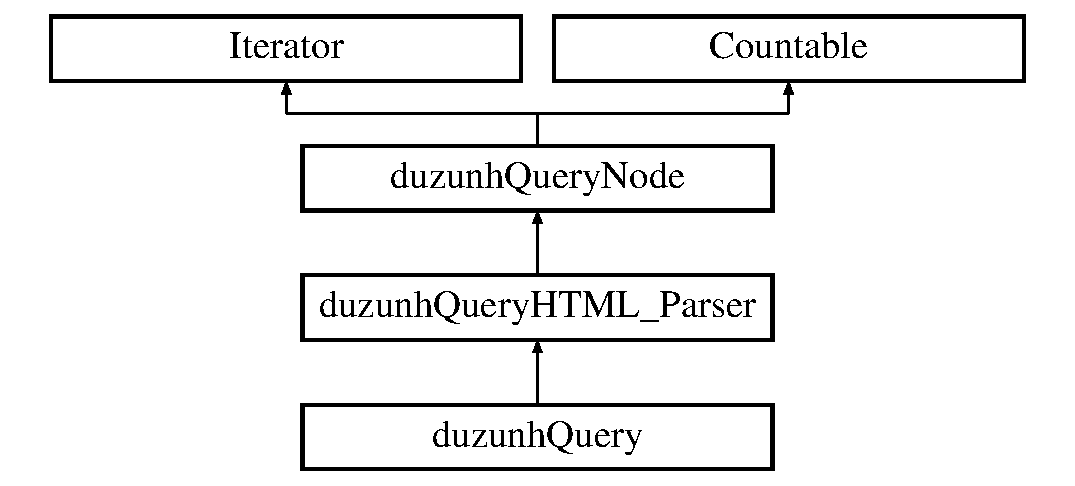
\includegraphics[height=4.000000cm]{classduzun_1_1hQuery_1_1HTML__Parser}
\end{center}
\end{figure}
\subsection*{Public Member Functions}
\begin{DoxyCompactItemize}
\item 
\mbox{\Hypertarget{classduzun_1_1hQuery_1_1HTML__Parser_a8cd9ada37e74d9f6796f47321e767e71}\label{classduzun_1_1hQuery_1_1HTML__Parser_a8cd9ada37e74d9f6796f47321e767e71}} 
{\bfseries \+\_\+\+\_\+get} (\$name)
\item 
\mbox{\Hypertarget{classduzun_1_1hQuery_1_1HTML__Parser_a290ba5ad97b5239956e46f78db375885}\label{classduzun_1_1hQuery_1_1HTML__Parser_a290ba5ad97b5239956e46f78db375885}} 
{\bfseries \+\_\+\+\_\+set} (\$name, \$value)
\item 
\mbox{\Hypertarget{classduzun_1_1hQuery_1_1HTML__Parser_abc2570255fe5c58bac0feaf9dc0825a7}\label{classduzun_1_1hQuery_1_1HTML__Parser_abc2570255fe5c58bac0feaf9dc0825a7}} 
{\bfseries location} (\$href=N\+U\+LL)
\item 
\mbox{\Hypertarget{classduzun_1_1hQuery_1_1HTML__Parser_a9ad05e36f124719ec0e3b95e0a49535c}\label{classduzun_1_1hQuery_1_1HTML__Parser_a9ad05e36f124719ec0e3b95e0a49535c}} 
\mbox{\hyperlink{classduzun_1_1hQuery_1_1HTML__Parser_a9ad05e36f124719ec0e3b95e0a49535c}{base\+U\+RI}} (\$href=N\+U\+LL)
\begin{DoxyCompactList}\small\item\em get/set base\+U\+RI \end{DoxyCompactList}\item 
\mbox{\Hypertarget{classduzun_1_1hQuery_1_1HTML__Parser_a930824078d127ded54c478740728d792}\label{classduzun_1_1hQuery_1_1HTML__Parser_a930824078d127ded54c478740728d792}} 
{\bfseries \+\_\+\+\_\+construct} (\$\mbox{\hyperlink{classduzun_1_1hQuery_1_1Node_a6a251f5f93690fabb794c673388dd49b}{html}}, \$idx=true)
\item 
\mbox{\Hypertarget{classduzun_1_1hQuery_1_1HTML__Parser_ae43028c71c0a83a9a961405e72b3a1a6}\label{classduzun_1_1hQuery_1_1HTML__Parser_ae43028c71c0a83a9a961405e72b3a1a6}} 
{\bfseries \+\_\+\+\_\+to\+String} ()
\item 
\mbox{\Hypertarget{classduzun_1_1hQuery_1_1HTML__Parser_aa87a97f9028342c5a0ca9701f4ff7259}\label{classduzun_1_1hQuery_1_1HTML__Parser_aa87a97f9028342c5a0ca9701f4ff7259}} 
{\bfseries url2abs} (\$url)
\item 
\mbox{\Hypertarget{classduzun_1_1hQuery_1_1HTML__Parser_a79488fa75219c031fb3b5c010c5112ee}\label{classduzun_1_1hQuery_1_1HTML__Parser_a79488fa75219c031fb3b5c010c5112ee}} 
{\bfseries strlen} ()
\item 
\mbox{\Hypertarget{classduzun_1_1hQuery_1_1HTML__Parser_a06489bb4d115433e9a162f75d4494fd2}\label{classduzun_1_1hQuery_1_1HTML__Parser_a06489bb4d115433e9a162f75d4494fd2}} 
{\bfseries substr} (\$start, \$length=N\+U\+LL)
\item 
\mbox{\Hypertarget{classduzun_1_1hQuery_1_1HTML__Parser_a1f96e82fbe66a54108e2e152dde3f3f3}\label{classduzun_1_1hQuery_1_1HTML__Parser_a1f96e82fbe66a54108e2e152dde3f3f3}} 
\mbox{\hyperlink{classduzun_1_1hQuery_1_1HTML__Parser_a1f96e82fbe66a54108e2e152dde3f3f3}{\+\_\+info}} ()
\begin{DoxyCompactList}\small\item\em This method is for debugging only. \end{DoxyCompactList}\item 
\mbox{\hyperlink{classduzun_1_1hQuery_1_1HTML__Parser_a3c297951a22371649ceebfc1888523ed}{has\+Class}} (\$id, \$cl)
\end{DoxyCompactItemize}
\subsection*{Static Public Member Functions}
\begin{DoxyCompactItemize}
\item 
\mbox{\Hypertarget{classduzun_1_1hQuery_1_1HTML__Parser_a98cf1892a2d6fcc550efb7f7d15ec719}\label{classduzun_1_1hQuery_1_1HTML__Parser_a98cf1892a2d6fcc550efb7f7d15ec719}} 
static {\bfseries get\+\_\+url\+\_\+base} (\$url, \$array=false)
\item 
\mbox{\Hypertarget{classduzun_1_1hQuery_1_1HTML__Parser_ac207a5ca705d907faf143dbab4a03867}\label{classduzun_1_1hQuery_1_1HTML__Parser_ac207a5ca705d907faf143dbab4a03867}} 
static {\bfseries get\+\_\+url\+\_\+path} (\$url)
\item 
static \mbox{\hyperlink{classduzun_1_1hQuery_1_1HTML__Parser_ae0f17bc6b740af406a317dc79ae09dbd}{is\+\_\+url\+\_\+path}} (\$path)
\item 
static \mbox{\hyperlink{classduzun_1_1hQuery_1_1HTML__Parser_a0649133c5b89b3b1692546e9fe4c2442}{is\+\_\+abs\+\_\+path}} (\$path)
\item 
static \mbox{\hyperlink{classduzun_1_1hQuery_1_1HTML__Parser_acbbb861c06ae362dac6e67e05d296385}{abs\+\_\+url}} (\$url, \$base)
\item 
\mbox{\Hypertarget{classduzun_1_1hQuery_1_1HTML__Parser_a53dbf11c4d369a2235d871c19a3a389d}\label{classduzun_1_1hQuery_1_1HTML__Parser_a53dbf11c4d369a2235d871c19a3a389d}} 
static {\bfseries detect\+\_\+charset} (\$str)
\end{DoxyCompactItemize}
\subsection*{Static Public Attributes}
\begin{DoxyCompactItemize}
\item 
\mbox{\Hypertarget{classduzun_1_1hQuery_1_1HTML__Parser_aced2d66ba9dfc865f88e644c2f2109b9}\label{classduzun_1_1hQuery_1_1HTML__Parser_aced2d66ba9dfc865f88e644c2f2109b9}} 
static {\bfseries \$del\+\_\+spaces} = false
\item 
\mbox{\Hypertarget{classduzun_1_1hQuery_1_1HTML__Parser_aa7e1d946650f5be17c708bdc547b47bd}\label{classduzun_1_1hQuery_1_1HTML__Parser_aa7e1d946650f5be17c708bdc547b47bd}} 
static {\bfseries \$case\+\_\+folding} = true
\item 
\mbox{\Hypertarget{classduzun_1_1hQuery_1_1HTML__Parser_ad6893025b0552db0488b86294e9f6036}\label{classduzun_1_1hQuery_1_1HTML__Parser_ad6893025b0552db0488b86294e9f6036}} 
static {\bfseries \$autoclose\+\_\+tags} = false
\item 
\mbox{\Hypertarget{classduzun_1_1hQuery_1_1HTML__Parser_a03b01800ba00cf4e32f225205d30b3b2}\label{classduzun_1_1hQuery_1_1HTML__Parser_a03b01800ba00cf4e32f225205d30b3b2}} 
static {\bfseries \$\+\_\+empty\+Tags} = array(\textquotesingle{}base\textquotesingle{},\textquotesingle{}meta\textquotesingle{},\textquotesingle{}link\textquotesingle{},\textquotesingle{}hr\textquotesingle{},\textquotesingle{}br\textquotesingle{},\textquotesingle{}basefont\textquotesingle{},\textquotesingle{}param\textquotesingle{},\textquotesingle{}img\textquotesingle{},\textquotesingle{}area\textquotesingle{},\textquotesingle{}input\textquotesingle{},\textquotesingle{}isindex\textquotesingle{},\textquotesingle{}col\textquotesingle{})
\item 
\mbox{\Hypertarget{classduzun_1_1hQuery_1_1HTML__Parser_ab04209a1c4d752d9b4e4f93e5e61b369}\label{classduzun_1_1hQuery_1_1HTML__Parser_ab04209a1c4d752d9b4e4f93e5e61b369}} 
static {\bfseries \$\+\_\+special\+Tags} = array(\textquotesingle{}-\/-\/\textquotesingle{}=$>$\textquotesingle{}-\/-\/\textquotesingle{}, \textquotesingle{}\mbox{[}C\+D\+A\+TA\mbox{[}\textquotesingle{}=$>$\textquotesingle{}\mbox{]}\mbox{]}\textquotesingle{})
\item 
\mbox{\Hypertarget{classduzun_1_1hQuery_1_1HTML__Parser_a2355aaddc0f7b4861269750ae7bccac2}\label{classduzun_1_1hQuery_1_1HTML__Parser_a2355aaddc0f7b4861269750ae7bccac2}} 
static {\bfseries \$\+\_\+unparsed\+Tags} = array(\textquotesingle{}style\textquotesingle{}, \textquotesingle{}script\textquotesingle{})
\item 
\mbox{\Hypertarget{classduzun_1_1hQuery_1_1HTML__Parser_a330e322fa6ec111cf2830520450699ed}\label{classduzun_1_1hQuery_1_1HTML__Parser_a330e322fa6ec111cf2830520450699ed}} 
static {\bfseries \$\+\_\+index\+\_\+attribs} = array(\textquotesingle{}href\textquotesingle{}, \textquotesingle{}src\textquotesingle{})
\item 
\mbox{\Hypertarget{classduzun_1_1hQuery_1_1HTML__Parser_a2726cbbeb2e78ac6ef9675e2f05d9d15}\label{classduzun_1_1hQuery_1_1HTML__Parser_a2726cbbeb2e78ac6ef9675e2f05d9d15}} 
static {\bfseries \$\+\_\+url\+\_\+attribs} = array(\textquotesingle{}href\textquotesingle{}=$>$\textquotesingle{}href\textquotesingle{}, \textquotesingle{}src\textquotesingle{}=$>$\textquotesingle{}src\textquotesingle{})
\end{DoxyCompactItemize}
\subsection*{Protected Member Functions}
\begin{DoxyCompactItemize}
\item 
\mbox{\Hypertarget{classduzun_1_1hQuery_1_1HTML__Parser_af71688120ebc569f1f927fd49a8d8a6d}\label{classduzun_1_1hQuery_1_1HTML__Parser_af71688120ebc569f1f927fd49a8d8a6d}} 
\mbox{\hyperlink{classduzun_1_1hQuery_1_1HTML__Parser_af71688120ebc569f1f927fd49a8d8a6d}{\+\_\+index\+\_\+comments\+\_\+html}} (\$o)
\begin{DoxyCompactList}\small\item\em Index comment tags position in source H\+T\+ML. \end{DoxyCompactList}\item 
\mbox{\Hypertarget{classduzun_1_1hQuery_1_1HTML__Parser_a998f520ac070759080bab2319a2e8066}\label{classduzun_1_1hQuery_1_1HTML__Parser_a998f520ac070759080bab2319a2e8066}} 
{\bfseries \+\_\+index\+\_\+all} ()
\item 
\mbox{\Hypertarget{classduzun_1_1hQuery_1_1HTML__Parser_aa20858a8076d9319423f2cdd6a8efb8c}\label{classduzun_1_1hQuery_1_1HTML__Parser_aa20858a8076d9319423f2cdd6a8efb8c}} 
{\bfseries \+\_\+get\+\_\+ctx} (\$ctx)
\item 
\mbox{\Hypertarget{classduzun_1_1hQuery_1_1HTML__Parser_ab03fc1cb5c169a2ee49354db13bed1a5}\label{classduzun_1_1hQuery_1_1HTML__Parser_ab03fc1cb5c169a2ee49354db13bed1a5}} 
{\bfseries \+\_\+find} (\$name, \$class=N\+U\+LL, \$\mbox{\hyperlink{classduzun_1_1hQuery_1_1Node_a530ab9e8edeb1e876b369dcb321208c0}{attr}}=N\+U\+LL, \$ctx=N\+U\+LL, \$rec=true)
\item 
\mbox{\Hypertarget{classduzun_1_1hQuery_1_1HTML__Parser_aaa094e6668fb9274baf23fe10639a568}\label{classduzun_1_1hQuery_1_1HTML__Parser_aaa094e6668fb9274baf23fe10639a568}} 
{\bfseries \+\_\+filter} (\$ids, \$name=N\+U\+LL, \$class=N\+U\+LL, \$\mbox{\hyperlink{classduzun_1_1hQuery_1_1Node_a530ab9e8edeb1e876b369dcb321208c0}{attr}}=N\+U\+LL, \$ctx=N\+U\+LL)
\item 
\mbox{\hyperlink{classduzun_1_1hQuery_1_1HTML__Parser_aa41f6709d61ef133065bf7fce7cc7ca7}{get\+\_\+aids\+\_\+by\+Attr}} (\$\mbox{\hyperlink{classduzun_1_1hQuery_1_1Node_a530ab9e8edeb1e876b369dcb321208c0}{attr}}, \$as\+\_\+keys=false, \$actx=N\+U\+LL)
\item 
\mbox{\hyperlink{classduzun_1_1hQuery_1_1HTML__Parser_aa15518a385a1acf4e2d174e2c2a1bbeb}{get\+\_\+aids\+\_\+by\+Class}} (\$cl, \$as\+\_\+keys=false, \$actx=N\+U\+LL)
\item 
\mbox{\Hypertarget{classduzun_1_1hQuery_1_1HTML__Parser_a15c2877b3fb48638f6b72ee63fba48b3}\label{classduzun_1_1hQuery_1_1HTML__Parser_a15c2877b3fb48638f6b72ee63fba48b3}} 
{\bfseries get\+\_\+aids\+\_\+by\+Class\+Attr} (\$cl, \$\mbox{\hyperlink{classduzun_1_1hQuery_1_1Node_a530ab9e8edeb1e876b369dcb321208c0}{attr}}, \$as\+\_\+keys=false, \$actx=N\+U\+LL)
\item 
\mbox{\hyperlink{classduzun_1_1hQuery_1_1HTML__Parser_aa52f76edd98bf62306b955d7b56bbd6d}{get\+\_\+ids\+\_\+by\+Aid}} (\$aid, \$sort=true, \$has\+\_\+keys=false)
\item 
\mbox{\Hypertarget{classduzun_1_1hQuery_1_1HTML__Parser_a0b9fb11d65dbb37c1d177cfebf94482b}\label{classduzun_1_1hQuery_1_1HTML__Parser_a0b9fb11d65dbb37c1d177cfebf94482b}} 
{\bfseries get\+\_\+ids\+\_\+by\+Attr} (\$\mbox{\hyperlink{classduzun_1_1hQuery_1_1Node_a530ab9e8edeb1e876b369dcb321208c0}{attr}}, \$sort=true)
\item 
\mbox{\Hypertarget{classduzun_1_1hQuery_1_1HTML__Parser_ab4169e8be484a407c4513c7c8522c178}\label{classduzun_1_1hQuery_1_1HTML__Parser_ab4169e8be484a407c4513c7c8522c178}} 
{\bfseries get\+\_\+ids\+\_\+by\+Class} (\$cl, \$sort=true)
\item 
\mbox{\Hypertarget{classduzun_1_1hQuery_1_1HTML__Parser_a75208660815f0ed326d35a573c392342}\label{classduzun_1_1hQuery_1_1HTML__Parser_a75208660815f0ed326d35a573c392342}} 
{\bfseries get\+\_\+ids\+\_\+by\+Class\+Attr} (\$cl, \$\mbox{\hyperlink{classduzun_1_1hQuery_1_1Node_a530ab9e8edeb1e876b369dcb321208c0}{attr}}, \$sort=true)
\item 
\mbox{\Hypertarget{classduzun_1_1hQuery_1_1HTML__Parser_a58399bccda24724da44503d4ee893037}\label{classduzun_1_1hQuery_1_1HTML__Parser_a58399bccda24724da44503d4ee893037}} 
{\bfseries get\+\_\+attr\+\_\+by\+Aid} (\$aid, \$to\+\_\+str=false)
\item 
\mbox{\Hypertarget{classduzun_1_1hQuery_1_1HTML__Parser_a831ff3d15436fd6a205b690711bc0fbe}\label{classduzun_1_1hQuery_1_1HTML__Parser_a831ff3d15436fd6a205b690711bc0fbe}} 
{\bfseries get\+\_\+attr\+\_\+by\+Id} (\$id, \$\mbox{\hyperlink{classduzun_1_1hQuery_1_1Node_a530ab9e8edeb1e876b369dcb321208c0}{attr}}=N\+U\+LL, \$to\+\_\+str=false)
\end{DoxyCompactItemize}
\subsection*{Protected Attributes}
\begin{DoxyCompactItemize}
\item 
\mbox{\Hypertarget{classduzun_1_1hQuery_1_1HTML__Parser_a9632d5ffbe240ddfceb2907ec1bb466b}\label{classduzun_1_1hQuery_1_1HTML__Parser_a9632d5ffbe240ddfceb2907ec1bb466b}} 
{\bfseries \$html} = \textquotesingle{}\textquotesingle{}
\item 
\mbox{\Hypertarget{classduzun_1_1hQuery_1_1HTML__Parser_acc311586bd5f116e1445daee32b43106}\label{classduzun_1_1hQuery_1_1HTML__Parser_acc311586bd5f116e1445daee32b43106}} 
{\bfseries \$tags}
\item 
\mbox{\Hypertarget{classduzun_1_1hQuery_1_1HTML__Parser_a78f5cd6a728948f51c4e9217c44cadbd}\label{classduzun_1_1hQuery_1_1HTML__Parser_a78f5cd6a728948f51c4e9217c44cadbd}} 
{\bfseries \$attrs}
\item 
\mbox{\Hypertarget{classduzun_1_1hQuery_1_1HTML__Parser_a715427f22a815ab55d57842605b152e0}\label{classduzun_1_1hQuery_1_1HTML__Parser_a715427f22a815ab55d57842605b152e0}} 
{\bfseries \$attribs}
\item 
\mbox{\Hypertarget{classduzun_1_1hQuery_1_1HTML__Parser_a09150535f5091307838eff1e739e1e0e}\label{classduzun_1_1hQuery_1_1HTML__Parser_a09150535f5091307838eff1e739e1e0e}} 
{\bfseries \$idx\+\_\+attr}
\item 
\mbox{\Hypertarget{classduzun_1_1hQuery_1_1HTML__Parser_ad16c379c796dfa21bd5b82cc0b8e4b11}\label{classduzun_1_1hQuery_1_1HTML__Parser_ad16c379c796dfa21bd5b82cc0b8e4b11}} 
{\bfseries \$tag\+\_\+idx}
\item 
\mbox{\Hypertarget{classduzun_1_1hQuery_1_1HTML__Parser_ac03f77f4e0bbb461b9ae262e9a445360}\label{classduzun_1_1hQuery_1_1HTML__Parser_ac03f77f4e0bbb461b9ae262e9a445360}} 
{\bfseries \$attr\+\_\+idx}
\item 
\mbox{\Hypertarget{classduzun_1_1hQuery_1_1HTML__Parser_ae13fed26c6cfa9facd202a9af5e4b108}\label{classduzun_1_1hQuery_1_1HTML__Parser_ae13fed26c6cfa9facd202a9af5e4b108}} 
{\bfseries \$class\+\_\+idx}
\item 
\mbox{\Hypertarget{classduzun_1_1hQuery_1_1HTML__Parser_a887889e1afb40b099373a36a86c3e731}\label{classduzun_1_1hQuery_1_1HTML__Parser_a887889e1afb40b099373a36a86c3e731}} 
{\bfseries \$o} = N\+U\+LL
\item 
\mbox{\Hypertarget{classduzun_1_1hQuery_1_1HTML__Parser_af1a756442c493295128612a15c5566ac}\label{classduzun_1_1hQuery_1_1HTML__Parser_af1a756442c493295128612a15c5566ac}} 
{\bfseries \$indexed} = false
\end{DoxyCompactItemize}
\subsection*{Static Protected Attributes}
\begin{DoxyCompactItemize}
\item 
\mbox{\Hypertarget{classduzun_1_1hQuery_1_1HTML__Parser_a12d98ca660edc18fe28145aaa2409e75}\label{classduzun_1_1hQuery_1_1HTML__Parser_a12d98ca660edc18fe28145aaa2409e75}} 
static {\bfseries \$\+\_\+tag\+I\+D\+\_\+first\+\_\+letter} = \textquotesingle{}a-\/zA-\/Z\+\_\+\textquotesingle{}
\item 
\mbox{\Hypertarget{classduzun_1_1hQuery_1_1HTML__Parser_ae23502b1388a96f576627de9b708700e}\label{classduzun_1_1hQuery_1_1HTML__Parser_ae23502b1388a96f576627de9b708700e}} 
static {\bfseries \$\+\_\+tag\+I\+D\+\_\+letters} = \textquotesingle{}a-\/zA-\/Z\+\_\+0-\/9\+:\textbackslash{}-\/\textquotesingle{}
\item 
\mbox{\Hypertarget{classduzun_1_1hQuery_1_1HTML__Parser_a0251a92e5f4478f7b487e79b28936543}\label{classduzun_1_1hQuery_1_1HTML__Parser_a0251a92e5f4478f7b487e79b28936543}} 
static {\bfseries \$\+\_\+icharset} = \textquotesingle{}U\+TF-\/8\textquotesingle{}
\end{DoxyCompactItemize}
\subsection*{Additional Inherited Members}


\subsection{Detailed Description}
H\+T\+ML Parser Class 

Definition at line 12 of file H\+T\+M\+L\+\_\+\+Parser.\+php.



\subsection{Member Function Documentation}
\mbox{\Hypertarget{classduzun_1_1hQuery_1_1HTML__Parser_acbbb861c06ae362dac6e67e05d296385}\label{classduzun_1_1hQuery_1_1HTML__Parser_acbbb861c06ae362dac6e67e05d296385}} 
\index{duzun\+::h\+Query\+::\+H\+T\+M\+L\+\_\+\+Parser@{duzun\+::h\+Query\+::\+H\+T\+M\+L\+\_\+\+Parser}!abs\+\_\+url@{abs\+\_\+url}}
\index{abs\+\_\+url@{abs\+\_\+url}!duzun\+::h\+Query\+::\+H\+T\+M\+L\+\_\+\+Parser@{duzun\+::h\+Query\+::\+H\+T\+M\+L\+\_\+\+Parser}}
\subsubsection{\texorpdfstring{abs\+\_\+url()}{abs\_url()}}
{\footnotesize\ttfamily static duzun\textbackslash{}h\+Query\textbackslash{}\+H\+T\+M\+L\+\_\+\+Parser\+::abs\+\_\+url (\begin{DoxyParamCaption}\item[{}]{\$url,  }\item[{}]{\$base }\end{DoxyParamCaption})\hspace{0.3cm}{\ttfamily [static]}}

Given a \$url (relative or absolute) and a \$base url, returns absolute url for \$url.


\begin{DoxyParams}[1]{Parameters}
string & {\em \$url} & -\/ relative or absolute U\+RL \\
\hline
string & {\em \$base} & -\/ Base U\+RL for \$url\\
\hline
\end{DoxyParams}
\begin{DoxyReturn}{Returns}
string absolute U\+RL for \$url 
\end{DoxyReturn}


Definition at line 228 of file H\+T\+M\+L\+\_\+\+Parser.\+php.

\mbox{\Hypertarget{classduzun_1_1hQuery_1_1HTML__Parser_aa41f6709d61ef133065bf7fce7cc7ca7}\label{classduzun_1_1hQuery_1_1HTML__Parser_aa41f6709d61ef133065bf7fce7cc7ca7}} 
\index{duzun\+::h\+Query\+::\+H\+T\+M\+L\+\_\+\+Parser@{duzun\+::h\+Query\+::\+H\+T\+M\+L\+\_\+\+Parser}!get\+\_\+aids\+\_\+by\+Attr@{get\+\_\+aids\+\_\+by\+Attr}}
\index{get\+\_\+aids\+\_\+by\+Attr@{get\+\_\+aids\+\_\+by\+Attr}!duzun\+::h\+Query\+::\+H\+T\+M\+L\+\_\+\+Parser@{duzun\+::h\+Query\+::\+H\+T\+M\+L\+\_\+\+Parser}}
\subsubsection{\texorpdfstring{get\+\_\+aids\+\_\+by\+Attr()}{get\_aids\_byAttr()}}
{\footnotesize\ttfamily duzun\textbackslash{}h\+Query\textbackslash{}\+H\+T\+M\+L\+\_\+\+Parser\+::get\+\_\+aids\+\_\+by\+Attr (\begin{DoxyParamCaption}\item[{}]{\$attr,  }\item[{}]{\$as\+\_\+keys = {\ttfamily false},  }\item[{}]{\$actx = {\ttfamily NULL} }\end{DoxyParamCaption})\hspace{0.3cm}{\ttfamily [protected]}}

\begin{DoxyReturn}{Returns}
\mbox{[}aids\mbox{]} 
\end{DoxyReturn}


Definition at line 732 of file H\+T\+M\+L\+\_\+\+Parser.\+php.

\mbox{\Hypertarget{classduzun_1_1hQuery_1_1HTML__Parser_aa15518a385a1acf4e2d174e2c2a1bbeb}\label{classduzun_1_1hQuery_1_1HTML__Parser_aa15518a385a1acf4e2d174e2c2a1bbeb}} 
\index{duzun\+::h\+Query\+::\+H\+T\+M\+L\+\_\+\+Parser@{duzun\+::h\+Query\+::\+H\+T\+M\+L\+\_\+\+Parser}!get\+\_\+aids\+\_\+by\+Class@{get\+\_\+aids\+\_\+by\+Class}}
\index{get\+\_\+aids\+\_\+by\+Class@{get\+\_\+aids\+\_\+by\+Class}!duzun\+::h\+Query\+::\+H\+T\+M\+L\+\_\+\+Parser@{duzun\+::h\+Query\+::\+H\+T\+M\+L\+\_\+\+Parser}}
\subsubsection{\texorpdfstring{get\+\_\+aids\+\_\+by\+Class()}{get\_aids\_byClass()}}
{\footnotesize\ttfamily duzun\textbackslash{}h\+Query\textbackslash{}\+H\+T\+M\+L\+\_\+\+Parser\+::get\+\_\+aids\+\_\+by\+Class (\begin{DoxyParamCaption}\item[{}]{\$cl,  }\item[{}]{\$as\+\_\+keys = {\ttfamily false},  }\item[{}]{\$actx = {\ttfamily NULL} }\end{DoxyParamCaption})\hspace{0.3cm}{\ttfamily [protected]}}

\begin{DoxyReturn}{Returns}
\$as\+\_\+keys ? \mbox{[}aid =$>$ id $\vert$ \mbox{[}ids\mbox{]}\mbox{]} \+: \mbox{[}aids\mbox{]} 
\end{DoxyReturn}


Definition at line 756 of file H\+T\+M\+L\+\_\+\+Parser.\+php.

\mbox{\Hypertarget{classduzun_1_1hQuery_1_1HTML__Parser_aa52f76edd98bf62306b955d7b56bbd6d}\label{classduzun_1_1hQuery_1_1HTML__Parser_aa52f76edd98bf62306b955d7b56bbd6d}} 
\index{duzun\+::h\+Query\+::\+H\+T\+M\+L\+\_\+\+Parser@{duzun\+::h\+Query\+::\+H\+T\+M\+L\+\_\+\+Parser}!get\+\_\+ids\+\_\+by\+Aid@{get\+\_\+ids\+\_\+by\+Aid}}
\index{get\+\_\+ids\+\_\+by\+Aid@{get\+\_\+ids\+\_\+by\+Aid}!duzun\+::h\+Query\+::\+H\+T\+M\+L\+\_\+\+Parser@{duzun\+::h\+Query\+::\+H\+T\+M\+L\+\_\+\+Parser}}
\subsubsection{\texorpdfstring{get\+\_\+ids\+\_\+by\+Aid()}{get\_ids\_byAid()}}
{\footnotesize\ttfamily duzun\textbackslash{}h\+Query\textbackslash{}\+H\+T\+M\+L\+\_\+\+Parser\+::get\+\_\+ids\+\_\+by\+Aid (\begin{DoxyParamCaption}\item[{}]{\$aid,  }\item[{}]{\$sort = {\ttfamily true},  }\item[{}]{\$has\+\_\+keys = {\ttfamily false} }\end{DoxyParamCaption})\hspace{0.3cm}{\ttfamily [protected]}}

\$has\+\_\+keys == true =$>$ \$aid == \mbox{[}aid=$>$\mbox{[}ids\mbox{]}\mbox{]} \$has\+\_\+keys == false =$>$ \$aid == \mbox{[}aids\mbox{]} 

Definition at line 797 of file H\+T\+M\+L\+\_\+\+Parser.\+php.

\mbox{\Hypertarget{classduzun_1_1hQuery_1_1HTML__Parser_a3c297951a22371649ceebfc1888523ed}\label{classduzun_1_1hQuery_1_1HTML__Parser_a3c297951a22371649ceebfc1888523ed}} 
\index{duzun\+::h\+Query\+::\+H\+T\+M\+L\+\_\+\+Parser@{duzun\+::h\+Query\+::\+H\+T\+M\+L\+\_\+\+Parser}!has\+Class@{has\+Class}}
\index{has\+Class@{has\+Class}!duzun\+::h\+Query\+::\+H\+T\+M\+L\+\_\+\+Parser@{duzun\+::h\+Query\+::\+H\+T\+M\+L\+\_\+\+Parser}}
\subsubsection{\texorpdfstring{has\+Class()}{hasClass()}}
{\footnotesize\ttfamily duzun\textbackslash{}h\+Query\textbackslash{}\+H\+T\+M\+L\+\_\+\+Parser\+::has\+Class (\begin{DoxyParamCaption}\item[{}]{\$id,  }\item[{}]{\$cl }\end{DoxyParamCaption})}

Checks whether \$this element/collection has a(ll) class(es).


\begin{DoxyParams}[1]{Parameters}
int | array | string | \mbox{\hyperlink{classduzun_1_1hQuery_1_1Node}{Node}} & {\em \$id} & -\/ The context to check \\
\hline
string | array & {\em \$cl} & -\/ class(es) to check \\
\hline
\end{DoxyParams}
\begin{DoxyReturn}{Returns}
false -\/ no class, 0 -\/ doesn\textquotesingle{}t have any class, true -\/ has class, \mbox{[}id =$>$ true\mbox{]} 
\end{DoxyReturn}


Definition at line 660 of file H\+T\+M\+L\+\_\+\+Parser.\+php.



References duzun\textbackslash{}h\+Query\textbackslash{}find().

\mbox{\Hypertarget{classduzun_1_1hQuery_1_1HTML__Parser_a0649133c5b89b3b1692546e9fe4c2442}\label{classduzun_1_1hQuery_1_1HTML__Parser_a0649133c5b89b3b1692546e9fe4c2442}} 
\index{duzun\+::h\+Query\+::\+H\+T\+M\+L\+\_\+\+Parser@{duzun\+::h\+Query\+::\+H\+T\+M\+L\+\_\+\+Parser}!is\+\_\+abs\+\_\+path@{is\+\_\+abs\+\_\+path}}
\index{is\+\_\+abs\+\_\+path@{is\+\_\+abs\+\_\+path}!duzun\+::h\+Query\+::\+H\+T\+M\+L\+\_\+\+Parser@{duzun\+::h\+Query\+::\+H\+T\+M\+L\+\_\+\+Parser}}
\subsubsection{\texorpdfstring{is\+\_\+abs\+\_\+path()}{is\_abs\_path()}}
{\footnotesize\ttfamily static duzun\textbackslash{}h\+Query\textbackslash{}\+H\+T\+M\+L\+\_\+\+Parser\+::is\+\_\+abs\+\_\+path (\begin{DoxyParamCaption}\item[{}]{\$path }\end{DoxyParamCaption})\hspace{0.3cm}{\ttfamily [static]}}

Check whether \$path is an absolute path.


\begin{DoxyParams}[1]{Parameters}
string & {\em \$path} & -\/ a path to check\\
\hline
\end{DoxyParams}
\begin{DoxyReturn}{Returns}
bool T\+R\+UE if \$path is an absolute path, F\+A\+L\+SE otherwise 
\end{DoxyReturn}


Definition at line 208 of file H\+T\+M\+L\+\_\+\+Parser.\+php.

\mbox{\Hypertarget{classduzun_1_1hQuery_1_1HTML__Parser_ae0f17bc6b740af406a317dc79ae09dbd}\label{classduzun_1_1hQuery_1_1HTML__Parser_ae0f17bc6b740af406a317dc79ae09dbd}} 
\index{duzun\+::h\+Query\+::\+H\+T\+M\+L\+\_\+\+Parser@{duzun\+::h\+Query\+::\+H\+T\+M\+L\+\_\+\+Parser}!is\+\_\+url\+\_\+path@{is\+\_\+url\+\_\+path}}
\index{is\+\_\+url\+\_\+path@{is\+\_\+url\+\_\+path}!duzun\+::h\+Query\+::\+H\+T\+M\+L\+\_\+\+Parser@{duzun\+::h\+Query\+::\+H\+T\+M\+L\+\_\+\+Parser}}
\subsubsection{\texorpdfstring{is\+\_\+url\+\_\+path()}{is\_url\_path()}}
{\footnotesize\ttfamily static duzun\textbackslash{}h\+Query\textbackslash{}\+H\+T\+M\+L\+\_\+\+Parser\+::is\+\_\+url\+\_\+path (\begin{DoxyParamCaption}\item[{}]{\$path }\end{DoxyParamCaption})\hspace{0.3cm}{\ttfamily [static]}}

Check whether \$path is a valid url.


\begin{DoxyParams}[1]{Parameters}
string & {\em \$path} & -\/ a path to check\\
\hline
\end{DoxyParams}
\begin{DoxyReturn}{Returns}
bool T\+R\+UE if \$path is a valid U\+RL, F\+A\+L\+SE otherwise 
\end{DoxyReturn}


Definition at line 197 of file H\+T\+M\+L\+\_\+\+Parser.\+php.



The documentation for this class was generated from the following file\+:\begin{DoxyCompactItemize}
\item 
src/h\+Query/H\+T\+M\+L\+\_\+\+Parser.\+php\end{DoxyCompactItemize}

\hypertarget{classduzun_1_1hQuery_1_1Node}{}\section{duzun\textbackslash{}h\+Query\textbackslash{}Node Class Reference}
\label{classduzun_1_1hQuery_1_1Node}\index{duzun\textbackslash{}h\+Query\textbackslash{}\+Node@{duzun\textbackslash{}h\+Query\textbackslash{}\+Node}}
Inheritance diagram for duzun\textbackslash{}h\+Query\textbackslash{}Node\+:\begin{figure}[H]
\begin{center}
\leavevmode
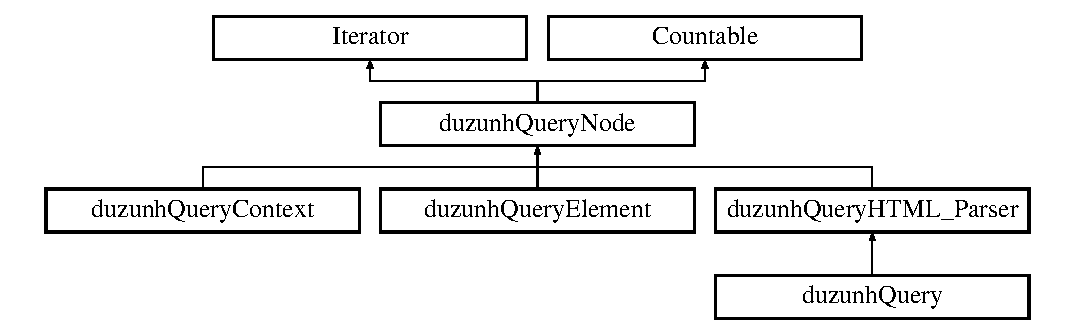
\includegraphics[height=4.000000cm]{classduzun_1_1hQuery_1_1Node}
\end{center}
\end{figure}
\subsection*{Public Member Functions}
\begin{DoxyCompactItemize}
\item 
\mbox{\hyperlink{classduzun_1_1hQuery_1_1Node_a530ab9e8edeb1e876b369dcb321208c0}{attr}} (\$attr=N\+U\+LL, \$to\+\_\+str=false)
\item 
\mbox{\Hypertarget{classduzun_1_1hQuery_1_1Node_a294afb6108604528401fbb1fa15b60cd}\label{classduzun_1_1hQuery_1_1Node_a294afb6108604528401fbb1fa15b60cd}} 
{\bfseries is\+\_\+empty} ()
\item 
\mbox{\Hypertarget{classduzun_1_1hQuery_1_1Node_a6e7b9f5f20609fc9a3e99ed52ec99910}\label{classduzun_1_1hQuery_1_1Node_a6e7b9f5f20609fc9a3e99ed52ec99910}} 
{\bfseries is\+Empty} ()
\item 
\mbox{\Hypertarget{classduzun_1_1hQuery_1_1Node_af530dc0a779ec124954c7c535262c104}\label{classduzun_1_1hQuery_1_1Node_af530dc0a779ec124954c7c535262c104}} 
{\bfseries is\+Doc} ()
\item 
\mbox{\hyperlink{classduzun_1_1hQuery_1_1Node_abd060c044c66e49189d8e4fb491f3b3d}{doc}} ()
\item 
\mbox{\hyperlink{classduzun_1_1hQuery_1_1Node_afec94d07336cc52b22aaf7b3cbcf7b27}{find}} (\$sel, \$\mbox{\hyperlink{classduzun_1_1hQuery_1_1Node_a530ab9e8edeb1e876b369dcb321208c0}{attr}}=N\+U\+LL)
\item 
\mbox{\Hypertarget{classduzun_1_1hQuery_1_1Node_a4736b811ac4bd8d83dad2ca2b6f68c58}\label{classduzun_1_1hQuery_1_1Node_a4736b811ac4bd8d83dad2ca2b6f68c58}} 
{\bfseries exclude} (\$sel, \$\mbox{\hyperlink{classduzun_1_1hQuery_1_1Node_a530ab9e8edeb1e876b369dcb321208c0}{attr}}=N\+U\+LL)
\item 
\mbox{\Hypertarget{classduzun_1_1hQuery_1_1Node_a73f08f113f804a35f5b0f9b8b8b40d09}\label{classduzun_1_1hQuery_1_1Node_a73f08f113f804a35f5b0f9b8b8b40d09}} 
{\bfseries \+\_\+\+\_\+to\+String} ()
\item 
\mbox{\hyperlink{classduzun_1_1hQuery_1_1Node_a6a251f5f93690fabb794c673388dd49b}{html}} (\$id=N\+U\+LL)
\item 
\mbox{\hyperlink{classduzun_1_1hQuery_1_1Node_ab3fb9d5a73f184da3a2a70d7ef73827c}{outer\+Html}} (\$id=N\+U\+LL)
\item 
\mbox{\hyperlink{classduzun_1_1hQuery_1_1Node_ad5395ffe77dd4f111fcc7f59d211fbfa}{text}} (\$id=N\+U\+LL)
\item 
\mbox{\hyperlink{classduzun_1_1hQuery_1_1Node_a82cc8fc0d4acd22bb0cd3fd50389f32d}{node\+Name}} (\$case\+Folding=N\+U\+LL, \$id=N\+U\+LL)
\item 
\mbox{\hyperlink{classduzun_1_1hQuery_1_1Node_a781a7e7f2540c4787915407279683e6f}{pos}} (\$restore=true)
\item 
\mbox{\Hypertarget{classduzun_1_1hQuery_1_1Node_a976e110ec37647d0f035b571a82e26f5}\label{classduzun_1_1hQuery_1_1Node_a976e110ec37647d0f035b571a82e26f5}} 
{\bfseries \+\_\+children} (\$ids=N\+U\+LL, \$n=N\+U\+LL)
\item 
\mbox{\Hypertarget{classduzun_1_1hQuery_1_1Node_a333630c8d0599d3db1aa004ef13bf210}\label{classduzun_1_1hQuery_1_1Node_a333630c8d0599d3db1aa004ef13bf210}} 
{\bfseries \+\_\+next} (\$ids=N\+U\+LL, \$n=0)
\item 
\mbox{\Hypertarget{classduzun_1_1hQuery_1_1Node_a0d542ee549f179d88b171e470d1b6eba}\label{classduzun_1_1hQuery_1_1Node_a0d542ee549f179d88b171e470d1b6eba}} 
{\bfseries \+\_\+prev} (\$ids=N\+U\+LL, \$n=0)
\item 
\mbox{\Hypertarget{classduzun_1_1hQuery_1_1Node_a3f1e8507527acd831a85b0fba9587188}\label{classduzun_1_1hQuery_1_1Node_a3f1e8507527acd831a85b0fba9587188}} 
{\bfseries \+\_\+all} (\$ids=N\+U\+LL)
\item 
\mbox{\Hypertarget{classduzun_1_1hQuery_1_1Node_a3d6209fff4e1d00a9feb2a4249dc91cf}\label{classduzun_1_1hQuery_1_1Node_a3d6209fff4e1d00a9feb2a4249dc91cf}} 
\mbox{\hyperlink{classduzun_1_1hQuery_1_1Node_a3d6209fff4e1d00a9feb2a4249dc91cf}{\+\_\+has}} (\$el, \$eq=false)
\begin{DoxyCompactList}\small\item\em \$el $<$ \$this, with \$eq == true -\/$>$ \$el $<$= \$this \end{DoxyCompactList}\item 
\mbox{\hyperlink{classduzun_1_1hQuery_1_1Node_a4419fd0f30515d4eb5cad2bfe7979754}{\+\_\+filter\+\_\+contains}} (\$el, \$eq=false)
\item 
\mbox{\Hypertarget{classduzun_1_1hQuery_1_1Node_a4038899dd8df17a881ac01516b3d6188}\label{classduzun_1_1hQuery_1_1Node_a4038899dd8df17a881ac01516b3d6188}} 
{\bfseries \+\_\+\+\_\+get} (\$name)
\item 
\mbox{\Hypertarget{classduzun_1_1hQuery_1_1Node_a9efe1826a38072a24f1575e6257cb4f3}\label{classduzun_1_1hQuery_1_1Node_a9efe1826a38072a24f1575e6257cb4f3}} 
{\bfseries \+\_\+\+\_\+set} (\$name, \$value)
\item 
\mbox{\Hypertarget{classduzun_1_1hQuery_1_1Node_a1aefdca7ea3af865a3a95abb27ef4e10}\label{classduzun_1_1hQuery_1_1Node_a1aefdca7ea3af865a3a95abb27ef4e10}} 
{\bfseries \+\_\+\+\_\+isset} (\$name)
\item 
\mbox{\Hypertarget{classduzun_1_1hQuery_1_1Node_ac717d6942600bbde289b452ae73d50c8}\label{classduzun_1_1hQuery_1_1Node_ac717d6942600bbde289b452ae73d50c8}} 
{\bfseries \+\_\+\+\_\+unset} (\$name)
\item 
\mbox{\Hypertarget{classduzun_1_1hQuery_1_1Node_a3385c7bac897f692816d0835a9161b81}\label{classduzun_1_1hQuery_1_1Node_a3385c7bac897f692816d0835a9161b81}} 
{\bfseries count} ()
\item 
\mbox{\Hypertarget{classduzun_1_1hQuery_1_1Node_a9f887f804779c4b8646030f1afc28063}\label{classduzun_1_1hQuery_1_1Node_a9f887f804779c4b8646030f1afc28063}} 
{\bfseries current} ()
\item 
\mbox{\Hypertarget{classduzun_1_1hQuery_1_1Node_a68e376130674fe8ef374d0173cd7ce2d}\label{classduzun_1_1hQuery_1_1Node_a68e376130674fe8ef374d0173cd7ce2d}} 
{\bfseries valid} ()
\item 
\mbox{\Hypertarget{classduzun_1_1hQuery_1_1Node_a6e140b7c620985244b6c10bafe80ce01}\label{classduzun_1_1hQuery_1_1Node_a6e140b7c620985244b6c10bafe80ce01}} 
{\bfseries key} ()
\item 
\mbox{\Hypertarget{classduzun_1_1hQuery_1_1Node_a927a7eaf8b0423ad6a4b38e05f3c0dbe}\label{classduzun_1_1hQuery_1_1Node_a927a7eaf8b0423ad6a4b38e05f3c0dbe}} 
{\bfseries next} ()
\item 
\mbox{\Hypertarget{classduzun_1_1hQuery_1_1Node_a9dea356d5b71a540cc3c60d9177e9113}\label{classduzun_1_1hQuery_1_1Node_a9dea356d5b71a540cc3c60d9177e9113}} 
{\bfseries prev} ()
\item 
\mbox{\Hypertarget{classduzun_1_1hQuery_1_1Node_a2d8632a843a59760e65183aa499b1137}\label{classduzun_1_1hQuery_1_1Node_a2d8632a843a59760e65183aa499b1137}} 
{\bfseries rewind} ()
\end{DoxyCompactItemize}
\subsection*{Static Public Member Functions}
\begin{DoxyCompactItemize}
\item 
static \mbox{\hyperlink{classduzun_1_1hQuery_1_1Node_a82f0739b0292cfb11570eeca08ac98c4}{html\+\_\+normal\+\_\+pseudo\+Class}} (\$p)
\item 
static \mbox{\hyperlink{classduzun_1_1hQuery_1_1Node_ac54f15080a896a8bad6bb21bddf56bac}{html\+\_\+selector2struc}} (\$sel)
\item 
\mbox{\Hypertarget{classduzun_1_1hQuery_1_1Node_ae0795251fe089b36b6c85f0ccec61cf5}\label{classduzun_1_1hQuery_1_1Node_ae0795251fe089b36b6c85f0ccec61cf5}} 
static {\bfseries html\+\_\+parse\+Attr\+Str} (\$str, \$case\+\_\+folding=true, \$extended=false)
\item 
\mbox{\Hypertarget{classduzun_1_1hQuery_1_1Node_a5ca45efa74a848a1e876191c1700246c}\label{classduzun_1_1hQuery_1_1Node_a5ca45efa74a848a1e876191c1700246c}} 
static {\bfseries html\+\_\+attr2str} (\$\mbox{\hyperlink{classduzun_1_1hQuery_1_1Node_a530ab9e8edeb1e876b369dcb321208c0}{attr}}, \$quote=\textquotesingle{}\char`\"{}\textquotesingle{}) 
\item 
\mbox{\Hypertarget{classduzun_1_1hQuery_1_1Node_a2cfdb22605901f90ca844b11d4d12a76}\label{classduzun_1_1hQuery_1_1Node_a2cfdb22605901f90ca844b11d4d12a76}} 
static {\bfseries parse\+C\+S\+Str} (\$str, \$case\+\_\+folding=true)
\item 
\mbox{\Hypertarget{classduzun_1_1hQuery_1_1Node_a2e1aa1fad388ee5e1e64f3bafcef245c}\label{classduzun_1_1hQuery_1_1Node_a2e1aa1fad388ee5e1e64f3bafcef245c}} 
static {\bfseries C\+S\+S\+Arr2\+Str} (\$css)
\item 
\mbox{\Hypertarget{classduzun_1_1hQuery_1_1Node_a57e45a91ed7e2a08f99b0e6a4bb9333b}\label{classduzun_1_1hQuery_1_1Node_a57e45a91ed7e2a08f99b0e6a4bb9333b}} 
static {\bfseries str\+\_\+range} (\$comp, \$\mbox{\hyperlink{classduzun_1_1hQuery_1_1Node_a781a7e7f2540c4787915407279683e6f}{pos}}=0, \$len=N\+U\+LL)
\item 
\mbox{\Hypertarget{classduzun_1_1hQuery_1_1Node_a4c19fe444170bee7077b9bb05abf4bd1}\label{classduzun_1_1hQuery_1_1Node_a4c19fe444170bee7077b9bb05abf4bd1}} 
static {\bfseries array\+\_\+select} (\$arr, \$keys, \$force\+\_\+null=false)
\item 
\mbox{\Hypertarget{classduzun_1_1hQuery_1_1Node_a85874b56f8ebd03b95766370af6d0b3b}\label{classduzun_1_1hQuery_1_1Node_a85874b56f8ebd03b95766370af6d0b3b}} 
static {\bfseries convert\+\_\+encoding} (\$a, \$to, \$from=N\+U\+LL)
\end{DoxyCompactItemize}
\subsection*{Public Attributes}
\begin{DoxyCompactItemize}
\item 
\mbox{\Hypertarget{classduzun_1_1hQuery_1_1Node_a26a33c519d62ecc351029fdad22038fd}\label{classduzun_1_1hQuery_1_1Node_a26a33c519d62ecc351029fdad22038fd}} 
const {\bfseries V\+E\+R\+S\+I\+ON} = \textquotesingle{}2.\+0.\+2\textquotesingle{}
\item 
\mbox{\Hypertarget{classduzun_1_1hQuery_1_1Node_a33c8622004dbbf3723c5c4af914f398e}\label{classduzun_1_1hQuery_1_1Node_a33c8622004dbbf3723c5c4af914f398e}} 
{\bfseries \$tag\+\_\+map}
\end{DoxyCompactItemize}
\subsection*{Static Public Attributes}
\begin{DoxyCompactItemize}
\item 
\mbox{\Hypertarget{classduzun_1_1hQuery_1_1Node_abca222acf298392097808df6ba2ec539}\label{classduzun_1_1hQuery_1_1Node_abca222acf298392097808df6ba2ec539}} 
static {\bfseries \$last\+\_\+http\+\_\+result}
\item 
\mbox{\Hypertarget{classduzun_1_1hQuery_1_1Node_a4fc24bd52aefff699526b031f1c579cf}\label{classduzun_1_1hQuery_1_1Node_a4fc24bd52aefff699526b031f1c579cf}} 
static {\bfseries \$selected\+\_\+doc} = N\+U\+LL
\item 
\mbox{\Hypertarget{classduzun_1_1hQuery_1_1Node_a8ed033358ffe33f07aa5a051379d7e71}\label{classduzun_1_1hQuery_1_1Node_a8ed033358ffe33f07aa5a051379d7e71}} 
static {\bfseries \$\+\_\+ar\+\_\+} = array()
\item 
\mbox{\Hypertarget{classduzun_1_1hQuery_1_1Node_ada2519db2120cc197d7dd5b1435d1727}\label{classduzun_1_1hQuery_1_1Node_ada2519db2120cc197d7dd5b1435d1727}} 
static {\bfseries \$\+\_\+mi\+\_\+} = P\+H\+P\+\_\+\+I\+N\+T\+\_\+\+M\+AX
\item 
\mbox{\Hypertarget{classduzun_1_1hQuery_1_1Node_acf39e90dde140c9a6fd672fb75c5df0c}\label{classduzun_1_1hQuery_1_1Node_acf39e90dde140c9a6fd672fb75c5df0c}} 
static {\bfseries \$\+\_\+nl\+\_\+} = N\+U\+LL
\item 
\mbox{\Hypertarget{classduzun_1_1hQuery_1_1Node_ab4aa94aeeb92d7ff8047b6d4401b0bc4}\label{classduzun_1_1hQuery_1_1Node_ab4aa94aeeb92d7ff8047b6d4401b0bc4}} 
static {\bfseries \$\+\_\+fl\+\_\+} = false
\item 
\mbox{\Hypertarget{classduzun_1_1hQuery_1_1Node_a8dc30378dc26cb361f9496fe0f495d84}\label{classduzun_1_1hQuery_1_1Node_a8dc30378dc26cb361f9496fe0f495d84}} 
static {\bfseries \$\+\_\+tr\+\_\+} = true
\end{DoxyCompactItemize}
\subsection*{Protected Member Functions}
\begin{DoxyCompactItemize}
\item 
\mbox{\Hypertarget{classduzun_1_1hQuery_1_1Node_aab1867ee99ebcff2d6d7c85e953ffeec}\label{classduzun_1_1hQuery_1_1Node_aab1867ee99ebcff2d6d7c85e953ffeec}} 
{\bfseries \+\_\+\+\_\+construct} (\$\mbox{\hyperlink{classduzun_1_1hQuery_1_1Node_abd060c044c66e49189d8e4fb491f3b3d}{doc}}, \$ids, \$is\+\_\+ctx=false)
\item 
\mbox{\hyperlink{classduzun_1_1hQuery_1_1Node_aec6b6185b6dfc245eca4364aa71000d1}{\+\_\+ctx\+\_\+ids}} (\$ids=N\+U\+LL)
\item 
\mbox{\hyperlink{classduzun_1_1hQuery_1_1Node_a4811866997e1bf7f09c1c5e05f37242d}{\+\_\+sub\+\_\+ids}} (\$eq=false)
\item 
\mbox{\hyperlink{classduzun_1_1hQuery_1_1Node_a3d9fe0b2908818d7d8feef2e55405d03}{\+\_\+doc\+\_\+ids}} (\$el, \$force\+\_\+array=true)
\item 
\mbox{\Hypertarget{classduzun_1_1hQuery_1_1Node_aefa8cc7452d31e55b577b9682a90220d}\label{classduzun_1_1hQuery_1_1Node_aefa8cc7452d31e55b577b9682a90220d}} 
{\bfseries \+\_\+my\+\_\+ids} (\$id=N\+U\+LL, \$keys=false)
\item 
\mbox{\Hypertarget{classduzun_1_1hQuery_1_1Node_a6225da6eb229da82c79b1ffbc644a984}\label{classduzun_1_1hQuery_1_1Node_a6225da6eb229da82c79b1ffbc644a984}} 
{\bfseries \+\_\+parent} (\$ids=N\+U\+LL, \$n=0)
\end{DoxyCompactItemize}
\subsection*{Static Protected Member Functions}
\begin{DoxyCompactItemize}
\item 
\mbox{\Hypertarget{classduzun_1_1hQuery_1_1Node_a6ac31707fc7d72635dc66e28af7955d2}\label{classduzun_1_1hQuery_1_1Node_a6ac31707fc7d72635dc66e28af7955d2}} 
static {\bfseries html\+\_\+find\+Tag\+Close} (\$str, \$p)
\end{DoxyCompactItemize}
\subsection*{Protected Attributes}
\begin{DoxyCompactItemize}
\item 
\mbox{\Hypertarget{classduzun_1_1hQuery_1_1Node_a7364e71ee9e2352d7d5b6d5d09fb5f1e}\label{classduzun_1_1hQuery_1_1Node_a7364e71ee9e2352d7d5b6d5d09fb5f1e}} 
{\bfseries \$\+\_\+prop} = array()
\item 
\mbox{\Hypertarget{classduzun_1_1hQuery_1_1Node_a81eeba47b20b3c4070c9823a3db24519}\label{classduzun_1_1hQuery_1_1Node_a81eeba47b20b3c4070c9823a3db24519}} 
{\bfseries \$doc}
\item 
\mbox{\Hypertarget{classduzun_1_1hQuery_1_1Node_aa84e29b3422dc9521e7a38ff0ac1657d}\label{classduzun_1_1hQuery_1_1Node_aa84e29b3422dc9521e7a38ff0ac1657d}} 
{\bfseries \$ids}
\item 
\mbox{\Hypertarget{classduzun_1_1hQuery_1_1Node_a3daf8fc1d60770e6baeb91989f7599ee}\label{classduzun_1_1hQuery_1_1Node_a3daf8fc1d60770e6baeb91989f7599ee}} 
{\bfseries \$exc}
\end{DoxyCompactItemize}


\subsection{Detailed Description}
Base class for H\+T\+ML Elements and Documents.

A\+PI Documentation at \href{https://duzun.github.io/hQuery.php}{\tt https\+://duzun.\+github.\+io/h\+Query.\+php}

M\+IT 

Definition at line 12 of file Node.\+php.



\subsection{Member Function Documentation}
\mbox{\Hypertarget{classduzun_1_1hQuery_1_1Node_aec6b6185b6dfc245eca4364aa71000d1}\label{classduzun_1_1hQuery_1_1Node_aec6b6185b6dfc245eca4364aa71000d1}} 
\index{duzun\+::h\+Query\+::\+Node@{duzun\+::h\+Query\+::\+Node}!\+\_\+ctx\+\_\+ids@{\+\_\+ctx\+\_\+ids}}
\index{\+\_\+ctx\+\_\+ids@{\+\_\+ctx\+\_\+ids}!duzun\+::h\+Query\+::\+Node@{duzun\+::h\+Query\+::\+Node}}
\subsubsection{\texorpdfstring{\+\_\+ctx\+\_\+ids()}{\_ctx\_ids()}}
{\footnotesize\ttfamily duzun\textbackslash{}h\+Query\textbackslash{}\+Node\+::\+\_\+ctx\+\_\+ids (\begin{DoxyParamCaption}\item[{}]{\$ids = {\ttfamily NULL} }\end{DoxyParamCaption})\hspace{0.3cm}{\ttfamily [protected]}}

Make a context array of ids\+: if x in \$ids \&\& exists y in \$ids such that x in y then del x from \$ids

\begin{DoxyReturn}{Returns}
array ids 
\end{DoxyReturn}


Definition at line 256 of file Node.\+php.



Referenced by duzun\textbackslash{}h\+Query\textbackslash{}\+Node\textbackslash{}\+\_\+has(), and duzun\textbackslash{}h\+Query\textbackslash{}\+Context\textbackslash{}intersect().

\mbox{\Hypertarget{classduzun_1_1hQuery_1_1Node_a3d9fe0b2908818d7d8feef2e55405d03}\label{classduzun_1_1hQuery_1_1Node_a3d9fe0b2908818d7d8feef2e55405d03}} 
\index{duzun\+::h\+Query\+::\+Node@{duzun\+::h\+Query\+::\+Node}!\+\_\+doc\+\_\+ids@{\+\_\+doc\+\_\+ids}}
\index{\+\_\+doc\+\_\+ids@{\+\_\+doc\+\_\+ids}!duzun\+::h\+Query\+::\+Node@{duzun\+::h\+Query\+::\+Node}}
\subsubsection{\texorpdfstring{\+\_\+doc\+\_\+ids()}{\_doc\_ids()}}
{\footnotesize\ttfamily duzun\textbackslash{}h\+Query\textbackslash{}\+Node\+::\+\_\+doc\+\_\+ids (\begin{DoxyParamCaption}\item[{}]{\$el,  }\item[{}]{\$force\+\_\+array = {\ttfamily true} }\end{DoxyParamCaption})\hspace{0.3cm}{\ttfamily [protected]}}

Get and Normalize ids of \$el

\begin{DoxyReturn}{Returns}
array ids 
\end{DoxyReturn}


Definition at line 299 of file Node.\+php.



References duzun\textbackslash{}h\+Query\textbackslash{}\+Node\textbackslash{}doc().



Referenced by duzun\textbackslash{}h\+Query\textbackslash{}\+Node\textbackslash{}\+\_\+filter\+\_\+contains(), duzun\textbackslash{}h\+Query\textbackslash{}\+Node\textbackslash{}\+\_\+has(), and duzun\textbackslash{}h\+Query\textbackslash{}\+Context\textbackslash{}intersect().

\mbox{\Hypertarget{classduzun_1_1hQuery_1_1Node_a4419fd0f30515d4eb5cad2bfe7979754}\label{classduzun_1_1hQuery_1_1Node_a4419fd0f30515d4eb5cad2bfe7979754}} 
\index{duzun\+::h\+Query\+::\+Node@{duzun\+::h\+Query\+::\+Node}!\+\_\+filter\+\_\+contains@{\+\_\+filter\+\_\+contains}}
\index{\+\_\+filter\+\_\+contains@{\+\_\+filter\+\_\+contains}!duzun\+::h\+Query\+::\+Node@{duzun\+::h\+Query\+::\+Node}}
\subsubsection{\texorpdfstring{\+\_\+filter\+\_\+contains()}{\_filter\_contains()}}
{\footnotesize\ttfamily duzun\textbackslash{}h\+Query\textbackslash{}\+Node\+::\+\_\+filter\+\_\+contains (\begin{DoxyParamCaption}\item[{}]{\$el,  }\item[{}]{\$eq = {\ttfamily false} }\end{DoxyParamCaption})}

Filter all ids of \$el that are contained in(side) \$this-\/$>$ids


\begin{DoxyParams}[1]{Parameters}
h\+Query\+\_\+\+Node | array & {\em \$el} & A node or list of ids \\
\hline
boolean & {\em \$eq} & if false, filter strict contents, otherwise \$el might be in \$this-\/$>$ids \\
\hline
\end{DoxyParams}
\begin{DoxyReturn}{Returns}
h\+Query\+\_\+\+Node$\vert$array same type as \$el 
\end{DoxyReturn}


Definition at line 591 of file Node.\+php.



References duzun\textbackslash{}h\+Query\textbackslash{}\+Node\textbackslash{}\+\_\+doc\+\_\+ids().

\mbox{\Hypertarget{classduzun_1_1hQuery_1_1Node_a4811866997e1bf7f09c1c5e05f37242d}\label{classduzun_1_1hQuery_1_1Node_a4811866997e1bf7f09c1c5e05f37242d}} 
\index{duzun\+::h\+Query\+::\+Node@{duzun\+::h\+Query\+::\+Node}!\+\_\+sub\+\_\+ids@{\+\_\+sub\+\_\+ids}}
\index{\+\_\+sub\+\_\+ids@{\+\_\+sub\+\_\+ids}!duzun\+::h\+Query\+::\+Node@{duzun\+::h\+Query\+::\+Node}}
\subsubsection{\texorpdfstring{\+\_\+sub\+\_\+ids()}{\_sub\_ids()}}
{\footnotesize\ttfamily duzun\textbackslash{}h\+Query\textbackslash{}\+Node\+::\+\_\+sub\+\_\+ids (\begin{DoxyParamCaption}\item[{}]{\$eq = {\ttfamily false} }\end{DoxyParamCaption})\hspace{0.3cm}{\ttfamily [protected]}}

Get all ids from inside of this element

\begin{DoxyReturn}{Returns}
array ids 
\end{DoxyReturn}


Definition at line 275 of file Node.\+php.



References duzun\textbackslash{}h\+Query\textbackslash{}\+Node\textbackslash{}doc().

\mbox{\Hypertarget{classduzun_1_1hQuery_1_1Node_a530ab9e8edeb1e876b369dcb321208c0}\label{classduzun_1_1hQuery_1_1Node_a530ab9e8edeb1e876b369dcb321208c0}} 
\index{duzun\+::h\+Query\+::\+Node@{duzun\+::h\+Query\+::\+Node}!attr@{attr}}
\index{attr@{attr}!duzun\+::h\+Query\+::\+Node@{duzun\+::h\+Query\+::\+Node}}
\subsubsection{\texorpdfstring{attr()}{attr()}}
{\footnotesize\ttfamily duzun\textbackslash{}h\+Query\textbackslash{}\+Node\+::attr (\begin{DoxyParamCaption}\item[{}]{\$attr = {\ttfamily NULL},  }\item[{}]{\$to\+\_\+str = {\ttfamily false} }\end{DoxyParamCaption})}

Get and attribute or all attributes of first element in the collection.


\begin{DoxyParams}[1]{Parameters}
string & {\em \$attr} & attribute name, or N\+U\+LL to get all \\
\hline
boolean & {\em \$to\+\_\+str} & When \$attr is N\+U\+LL, if true, get the list of attributes as string \\
\hline
\end{DoxyParams}
\begin{DoxyReturn}{Returns}
array$\vert$string If no \$attr, return a list of attributes, or attribute\textquotesingle{}s value otherwise. 
\end{DoxyReturn}


Definition at line 62 of file Node.\+php.



References duzun\textbackslash{}h\+Query\textbackslash{}\+Node\textbackslash{}doc().

\mbox{\Hypertarget{classduzun_1_1hQuery_1_1Node_abd060c044c66e49189d8e4fb491f3b3d}\label{classduzun_1_1hQuery_1_1Node_abd060c044c66e49189d8e4fb491f3b3d}} 
\index{duzun\+::h\+Query\+::\+Node@{duzun\+::h\+Query\+::\+Node}!doc@{doc}}
\index{doc@{doc}!duzun\+::h\+Query\+::\+Node@{duzun\+::h\+Query\+::\+Node}}
\subsubsection{\texorpdfstring{doc()}{doc()}}
{\footnotesize\ttfamily duzun\textbackslash{}h\+Query\textbackslash{}\+Node\+::doc (\begin{DoxyParamCaption}{ }\end{DoxyParamCaption})}

Get parent doc of this node.

\begin{DoxyReturn}{Returns}
\mbox{\hyperlink{classduzun_1_1hQuery}{h\+Query}} 
\end{DoxyReturn}


Definition at line 88 of file Node.\+php.



Referenced by duzun\textbackslash{}h\+Query\textbackslash{}\+Node\textbackslash{}\+\_\+doc\+\_\+ids(), duzun\textbackslash{}h\+Query\textbackslash{}\+Node\textbackslash{}\+\_\+sub\+\_\+ids(), duzun\textbackslash{}h\+Query\textbackslash{}\+Node\textbackslash{}attr(), duzun\textbackslash{}h\+Query\textbackslash{}\+Node\textbackslash{}find(), duzun\textbackslash{}h\+Query\textbackslash{}\+Element\textbackslash{}has\+Class(), duzun\textbackslash{}h\+Query\textbackslash{}\+Node\textbackslash{}node\+Name(), and duzun\textbackslash{}h\+Query\textbackslash{}\+Node\textbackslash{}outer\+Html().

\mbox{\Hypertarget{classduzun_1_1hQuery_1_1Node_afec94d07336cc52b22aaf7b3cbcf7b27}\label{classduzun_1_1hQuery_1_1Node_afec94d07336cc52b22aaf7b3cbcf7b27}} 
\index{duzun\+::h\+Query\+::\+Node@{duzun\+::h\+Query\+::\+Node}!find@{find}}
\index{find@{find}!duzun\+::h\+Query\+::\+Node@{duzun\+::h\+Query\+::\+Node}}
\subsubsection{\texorpdfstring{find()}{find()}}
{\footnotesize\ttfamily duzun\textbackslash{}h\+Query\textbackslash{}\+Node\+::find (\begin{DoxyParamCaption}\item[{}]{\$sel,  }\item[{}]{\$attr = {\ttfamily NULL} }\end{DoxyParamCaption})}

Finds a collection of nodes inside current document/context (similar to j\+Query.\+fn.\+find()).


\begin{DoxyParams}[1]{Parameters}
string & {\em \$sel} & -\/ A valid C\+SS selector (some pseudo-\/selectors supported). \\
\hline
array | string & {\em \$attr} & -\/ O\+P\+T\+I\+O\+N\+AL attributes as string or key-\/value pairs. \\
\hline
h\+Query\+\_\+\+Node & {\em \$ctx} & -\/ O\+P\+T\+I\+O\+N\+AL the context where to search. If omitted, \$this is used.\\
\hline
\end{DoxyParams}
\begin{DoxyReturn}{Returns}
h\+Query\+\_\+\+Element collection of matched elements or N\+U\+LL 
\end{DoxyReturn}


Definition at line 101 of file Node.\+php.



References duzun\textbackslash{}h\+Query\textbackslash{}\+Node\textbackslash{}doc().

\mbox{\Hypertarget{classduzun_1_1hQuery_1_1Node_a6a251f5f93690fabb794c673388dd49b}\label{classduzun_1_1hQuery_1_1Node_a6a251f5f93690fabb794c673388dd49b}} 
\index{duzun\+::h\+Query\+::\+Node@{duzun\+::h\+Query\+::\+Node}!html@{html}}
\index{html@{html}!duzun\+::h\+Query\+::\+Node@{duzun\+::h\+Query\+::\+Node}}
\subsubsection{\texorpdfstring{html()}{html()}}
{\footnotesize\ttfamily duzun\textbackslash{}h\+Query\textbackslash{}\+Node\+::html (\begin{DoxyParamCaption}\item[{}]{\$id = {\ttfamily NULL} }\end{DoxyParamCaption})}

\begin{DoxyReturn}{Returns}
string .inner\+H\+T\+ML 
\end{DoxyReturn}


Definition at line 142 of file Node.\+php.



Referenced by duzun\textbackslash{}h\+Query\textbackslash{}\+Node\textbackslash{}text().

\mbox{\Hypertarget{classduzun_1_1hQuery_1_1Node_a82f0739b0292cfb11570eeca08ac98c4}\label{classduzun_1_1hQuery_1_1Node_a82f0739b0292cfb11570eeca08ac98c4}} 
\index{duzun\+::h\+Query\+::\+Node@{duzun\+::h\+Query\+::\+Node}!html\+\_\+normal\+\_\+pseudo\+Class@{html\+\_\+normal\+\_\+pseudo\+Class}}
\index{html\+\_\+normal\+\_\+pseudo\+Class@{html\+\_\+normal\+\_\+pseudo\+Class}!duzun\+::h\+Query\+::\+Node@{duzun\+::h\+Query\+::\+Node}}
\subsubsection{\texorpdfstring{html\+\_\+normal\+\_\+pseudo\+Class()}{html\_normal\_pseudoClass()}}
{\footnotesize\ttfamily static duzun\textbackslash{}h\+Query\textbackslash{}\+Node\+::html\+\_\+normal\+\_\+pseudo\+Class (\begin{DoxyParamCaption}\item[{}]{\$p }\end{DoxyParamCaption})\hspace{0.3cm}{\ttfamily [static]}}

Normalize a C\+SS selector pseudo-\/class string. ( int, string or array(name =$>$ value) )

\begin{DoxyReturn}{Returns}
int$\vert$array 
\end{DoxyReturn}


Definition at line 663 of file Node.\+php.

\mbox{\Hypertarget{classduzun_1_1hQuery_1_1Node_ac54f15080a896a8bad6bb21bddf56bac}\label{classduzun_1_1hQuery_1_1Node_ac54f15080a896a8bad6bb21bddf56bac}} 
\index{duzun\+::h\+Query\+::\+Node@{duzun\+::h\+Query\+::\+Node}!html\+\_\+selector2struc@{html\+\_\+selector2struc}}
\index{html\+\_\+selector2struc@{html\+\_\+selector2struc}!duzun\+::h\+Query\+::\+Node@{duzun\+::h\+Query\+::\+Node}}
\subsubsection{\texorpdfstring{html\+\_\+selector2struc()}{html\_selector2struc()}}
{\footnotesize\ttfamily static duzun\textbackslash{}h\+Query\textbackslash{}\+Node\+::html\+\_\+selector2struc (\begin{DoxyParamCaption}\item[{}]{\$sel }\end{DoxyParamCaption})\hspace{0.3cm}{\ttfamily [static]}}

Parse a selector string into an array structure.

tn1\+::id1 .cl1.\+cl2\+:first tn2\+:5 , tn3.\+cl3 tn4\+::id2\+:eq(-\/1) $>$ tn5\+:last-\/child $>$ tn6\+:lt(3) --$>$ \mbox{[} \mbox{[} \mbox{[}\{ n\+: \char`\"{}tn1\char`\"{}, i\+: \char`\"{}id1\char`\"{}, c\+: \mbox{[}\mbox{]}, p\+: \mbox{[}\mbox{]} \}\mbox{]}, \mbox{[}\{ n\+: N\+U\+LL, i\+: N\+U\+LL, c\+: \mbox{[}\char`\"{}cl1\char`\"{},\char`\"{}cl2\char`\"{}\mbox{]}, p\+: \mbox{[}0\mbox{]} \}\mbox{]}, \mbox{[}\{ n\+: \char`\"{}tn2\char`\"{}, i\+: N\+U\+LL, c\+: \mbox{[}\mbox{]}, p\+: \mbox{[}5\mbox{]} \}\mbox{]} \mbox{]} , \mbox{[} \mbox{[}\{ n\+: \char`\"{}tn3\char`\"{}, i\+: N\+U\+LL, c\+: \mbox{[}\char`\"{}cl3\char`\"{}\mbox{]}, p\+: \mbox{[}\mbox{]} \}\mbox{]}, \mbox{[} \{ n\+: \char`\"{}tn4\char`\"{}, i\+: \char`\"{}id2\char`\"{}, c\+: \mbox{[}\mbox{]}, p\+: \mbox{[}-\/1\mbox{]} \}, \{ n\+: \char`\"{}tn5\char`\"{}, i\+: N\+U\+LL , c\+: \mbox{[}\mbox{]}, p\+: \mbox{[}-\/1\mbox{]} \}, \{ n\+: \char`\"{}tn6\char`\"{}, i\+: N\+U\+LL , c\+: \mbox{[}\mbox{]}, p\+: \mbox{[}\char`\"{}$<$3\char`\"{}\mbox{]} \} \mbox{]} \mbox{]} \mbox{]}

\begin{DoxyReturn}{Returns}
array 
\end{DoxyReturn}


Definition at line 723 of file Node.\+php.

\mbox{\Hypertarget{classduzun_1_1hQuery_1_1Node_a82cc8fc0d4acd22bb0cd3fd50389f32d}\label{classduzun_1_1hQuery_1_1Node_a82cc8fc0d4acd22bb0cd3fd50389f32d}} 
\index{duzun\+::h\+Query\+::\+Node@{duzun\+::h\+Query\+::\+Node}!node\+Name@{node\+Name}}
\index{node\+Name@{node\+Name}!duzun\+::h\+Query\+::\+Node@{duzun\+::h\+Query\+::\+Node}}
\subsubsection{\texorpdfstring{node\+Name()}{nodeName()}}
{\footnotesize\ttfamily duzun\textbackslash{}h\+Query\textbackslash{}\+Node\+::node\+Name (\begin{DoxyParamCaption}\item[{}]{\$case\+Folding = {\ttfamily NULL},  }\item[{}]{\$id = {\ttfamily NULL} }\end{DoxyParamCaption})}

\begin{DoxyReturn}{Returns}
string .node\+Name 
\end{DoxyReturn}


Definition at line 194 of file Node.\+php.



References duzun\textbackslash{}h\+Query\textbackslash{}\+Node\textbackslash{}doc().

\mbox{\Hypertarget{classduzun_1_1hQuery_1_1Node_ab3fb9d5a73f184da3a2a70d7ef73827c}\label{classduzun_1_1hQuery_1_1Node_ab3fb9d5a73f184da3a2a70d7ef73827c}} 
\index{duzun\+::h\+Query\+::\+Node@{duzun\+::h\+Query\+::\+Node}!outer\+Html@{outer\+Html}}
\index{outer\+Html@{outer\+Html}!duzun\+::h\+Query\+::\+Node@{duzun\+::h\+Query\+::\+Node}}
\subsubsection{\texorpdfstring{outer\+Html()}{outerHtml()}}
{\footnotesize\ttfamily duzun\textbackslash{}h\+Query\textbackslash{}\+Node\+::outer\+Html (\begin{DoxyParamCaption}\item[{}]{\$id = {\ttfamily NULL} }\end{DoxyParamCaption})}

\begin{DoxyReturn}{Returns}
string .outer\+Html 
\end{DoxyReturn}


Definition at line 165 of file Node.\+php.



References duzun\textbackslash{}h\+Query\textbackslash{}\+Node\textbackslash{}doc().

\mbox{\Hypertarget{classduzun_1_1hQuery_1_1Node_a781a7e7f2540c4787915407279683e6f}\label{classduzun_1_1hQuery_1_1Node_a781a7e7f2540c4787915407279683e6f}} 
\index{duzun\+::h\+Query\+::\+Node@{duzun\+::h\+Query\+::\+Node}!pos@{pos}}
\index{pos@{pos}!duzun\+::h\+Query\+::\+Node@{duzun\+::h\+Query\+::\+Node}}
\subsubsection{\texorpdfstring{pos()}{pos()}}
{\footnotesize\ttfamily duzun\textbackslash{}h\+Query\textbackslash{}\+Node\+::pos (\begin{DoxyParamCaption}\item[{}]{\$restore = {\ttfamily true} }\end{DoxyParamCaption})}

Get string offset of the first/current element in the source H\+T\+ML document.

 Contents of \#test  $\vert$ \mbox{\hyperlink{classduzun_1_1hQuery_1_1Node_a781a7e7f2540c4787915407279683e6f}{pos()}}


\begin{DoxyParams}[1]{Parameters}
bool & {\em \$restore} & -\/ if true, restore internal pointer to previous position\\
\hline
\end{DoxyParams}
\begin{DoxyReturn}{Returns}
int 
\end{DoxyReturn}


Definition at line 237 of file Node.\+php.

\mbox{\Hypertarget{classduzun_1_1hQuery_1_1Node_ad5395ffe77dd4f111fcc7f59d211fbfa}\label{classduzun_1_1hQuery_1_1Node_ad5395ffe77dd4f111fcc7f59d211fbfa}} 
\index{duzun\+::h\+Query\+::\+Node@{duzun\+::h\+Query\+::\+Node}!text@{text}}
\index{text@{text}!duzun\+::h\+Query\+::\+Node@{duzun\+::h\+Query\+::\+Node}}
\subsubsection{\texorpdfstring{text()}{text()}}
{\footnotesize\ttfamily duzun\textbackslash{}h\+Query\textbackslash{}\+Node\+::text (\begin{DoxyParamCaption}\item[{}]{\$id = {\ttfamily NULL} }\end{DoxyParamCaption})}

\begin{DoxyReturn}{Returns}
string .inner\+Text 
\end{DoxyReturn}


Definition at line 187 of file Node.\+php.



References duzun\textbackslash{}h\+Query\textbackslash{}\+Node\textbackslash{}html().



The documentation for this class was generated from the following file\+:\begin{DoxyCompactItemize}
\item 
src/h\+Query/Node.\+php\end{DoxyCompactItemize}

%--- End generated contents ---

% Index
\backmatter
\newpage
\phantomsection
\clearemptydoublepage
\addcontentsline{toc}{chapter}{Index}
\printindex

\end{document}
